% ============================================================
% Curriculum vs Mixed-Batch Training in MARL for Urban Driving
% Bachelor's thesis (triennale) — ~60 pages, English
% Build: pdflatex main_en + biber main_en + pdflatex x2
% ============================================================
\documentclass[12pt,a4paper,oneside]{report}

% --- Encoding & language ---
\usepackage[utf8]{inputenc}
\usepackage[T1]{fontenc}
\usepackage{lmodern}
\usepackage[english]{babel}
\usepackage{csquotes}

% --- Layout ---
\usepackage[a4paper,margin=2.5cm]{geometry}
\usepackage{setspace}
\onehalfspacing
\usepackage{microtype}

% --- Math, tables, units, figures ---
\usepackage{amsmath,amssymb}
\usepackage{graphicx}
\graphicspath{{figures/}}
\usepackage{booktabs}
\usepackage{longtable}
\usepackage{verbatim}
\usepackage{siunitx}
\usepackage{tikz}
\usetikzlibrary{positioning,arrows.meta}

% --- Bibliography ---
\usepackage[style=numeric-comp,sorting=none,backend=biber]{biblatex}
\addbibresource{bibliography.bib}

% --- Colors, links, cross-references (hyperref near the end) ---
\usepackage{xcolor}
\usepackage[hidelinks]{hyperref}
\usepackage[capitalise,noabbrev]{cleveref}

% --- Working notes: red TODO markers, remove before submission ---
\newcommand{\todo}[1]{\textcolor{red}{\textbf{[TODO: #1]}}}

% ============================================================
\begin{document}

% Front matter: roman page numbers (title page counts as i);
% arabic restarts at Chapter 1. Also removes the hyperref
% "duplicate destination page.1" warning.
\pagenumbering{roman}

% ----------------- Title page (official UniMarconi template) -----
% Replicates Frontespizio.doc (Downloads, converted 2026-07-19): logo,
% university heading, department / degree lines, quoted italic title,
% Relatore/Candidato two-column block, academic year. Blank fields keep
% red \todo markers until filled.
\begin{titlepage}
  \centering
  
\includegraphics[height=2.0cm]{logo_unimarconi}\par
  \vspace{1.5cm}
  {\large\bfseries UNIVERSIT\`A DEGLI STUDI GUGLIELMO MARCONI\par}
  \vspace{0.9cm}
  {\bfseries DIPARTIMENTO DI \todo{dipartimento}\par}
  \vspace{0.9cm}
  {\bfseries CORSO DI LAUREA IN \todo{corso di laurea}\par}
  \vfill
  {\Large\itshape ``Curriculum versus Mixed-Batch Training in
  Multi-Agent Reinforcement Learning for Urban Autonomous
  Driving''\par}
  \vfill
  {\large
   \begin{minipage}[t]{0.50\textwidth}
     \raggedright
     Relatore:\\[1.2em]
     Prof.\ \todo{nome relatore}
   \end{minipage}%
   \hfill
   \begin{minipage}[t]{0.40\textwidth}
     \raggedright
     Candidato:\\[1.2em]
     \todo{nome candidato}
   \end{minipage}\par}
  \vfill
  {\footnotesize ANNO ACCADEMICO \todo{20XX/20XX}\par}
\end{titlepage}
% titlepage resets the page counter; account for the title page as i
\setcounter{page}{2}

% ----------------- Abstract ---------------------------------
% Manual abstract page: the report-class abstract environment wraps a
% titlepage and resets the page counter, breaking front-matter numbering.
\clearpage
\null\vfil
\begin{center}%
  \bfseries \abstractname
\end{center}
The order in which training tasks are presented is a design decision in
reinforcement learning whose effects are rarely isolated in multi-agent
settings. This thesis compares curriculum learning (easy-to-hard
progression gated on measured competence) against mixed-batch training
(uniform interleaving of all difficulties) for urban driving in CARLA,
with six agents --- three vehicles and three pedestrians --- learning
simultaneously in one shared world under MAPPO with centralized critics.
A $2\times2$ seed-paired campaign crosses the two regimes with two
critic encoders (MLP and GNN) at three million steps per run, on a
platform hardened by a gate-driven development protocol, measured under
a strict success criterion, with same-seed replicates providing an
explicit noise band.

Task ordering did not accelerate early learning: all cells crossed the
same competence thresholds at the same step counts. It instead selected
what the policy became. Under the MLP critic, the curriculum produced a
cautious, stalling-prone driver and batch a fast, colliding one; the
curriculum led by $+18.5$ percentage points of vehicle success at
evaluation, consistently across scenarios. Under the GNN critic the
in-domain effect vanished ($-0.1$\,pp) --- a strong
architecture$\times$regime interaction --- while the same encoder
markedly improved the batch cell. The only component that replicated
across both architectures is the curriculum's advantage on a town never
seen in training ($+19.0$ and $+10.0$\,pp), against the intuition that
broader coverage buys robustness. Pedestrians were bounded by route
feasibility rather than by regime. Task ordering, in this setting, is an
equilibrium selector whose in-domain payoff depends on value estimation
--- and whose portable benefit is generalization.
\par\vfil\null

\tableofcontents

% ----------------- Acronyms ---------------------------------
\chapter*{Acronyms}
\addcontentsline{toc}{chapter}{Acronyms}
\begin{tabular}{ll}
CTDE  & Centralized Training with Decentralized Execution \\
GAE   & Generalized Advantage Estimation \\
GNN   & Graph Neural Network \\
MAPPO & Multi-Agent Proximal Policy Optimization \\
MARL  & Multi-Agent Reinforcement Learning \\
MLP   & Multi-Layer Perceptron \\
NPC   & Non-Player Character (scripted traffic participant) \\
PPO   & Proximal Policy Optimization \\
RL    & Reinforcement Learning \\
SR    & Success Rate \\
TM    & (CARLA) Traffic Manager \\
\end{tabular}

% ----------------- Chapters ---------------------------------
\clearpage
\pagenumbering{arabic}
% ============================================================
% Chapter 1 — Introduction (target 4–5 pp)
% Status: FULL DRAFT 2026-07-17, written fresh against the final
% campaign results (the 2026-07-06 chat draft was never recovered;
% if it resurfaces, merge selectively).
% ============================================================
\chapter{Introduction}
\label{ch:intro}

\section{Motivation}
\label{sec:motivation}

Reinforcement learning trains control policies by trial and error, and
in any non-trivial domain the designer faces a scheduling question
before the first gradient step: when the tasks to master span a range of
difficulty, \emph{in what order should they be presented}? Two answers
are natural. \emph{Curriculum learning} presents tasks from easy to
hard, echoing human pedagogy: build competence where success is
reachable, then extend it. \emph{Mixed training} presents everything
from the start --- the direct analogue of training on a shuffled
dataset, which is the unquestioned default in supervised learning. Both
strategies consume the same budget; choosing between them is, in
principle, free. If the choice changes what the learned policy does, it
is among the cheapest levers a designer controls --- and one of the
least characterized, especially in multi-agent settings, where most of
the curriculum literature's assumptions (single learner, sparse rewards,
stationary environment) do not hold.

Urban autonomous driving is a demanding place to ask the question.
It offers a natural difficulty axis (route length), heterogeneous
agents with different embodiments and constraints (vehicles and
pedestrians), a built-in tension between performance and safety
(faster policies complete more routes and hit more things), and a
canonical out-of-distribution test (drive on a town never seen in
training). It is also intrinsically multi-agent: policies do not just
share a world, they shape each other's environment while learning ---
the non-stationarity at the heart of multi-agent reinforcement
learning. This thesis asks the ordering question there, and treats the
training regime itself as the experimental variable.

\section{Research Question and Hypotheses}
\label{sec:rq}

\begin{quote}
  \emph{Does curriculum learning from easy to medium to hard produce
  measurably different multi-agent driving behaviour than mixed-batch
  training, at equal training budget?}
\end{quote}

The question is deliberately about \emph{behaviour}, not about a single
success-rate leaderboard: the comparison is evaluated along four axes
--- sample efficiency, final performance with its failure composition,
within-run training dynamics, and map generalization --- always
separately for vehicles and pedestrians. Three falsifiable hypotheses
structure the analysis:

\begin{itemize}
  \item \textbf{H1 (curriculum).} Staged exposure yields better early
        sample efficiency --- easy tasks provide reachable success to
        bootstrap from --- with a known risk of plateauing on, or
        forgetting, harder tasks introduced late.
  \item \textbf{H2 (mixed).} Uniform exposure covers the full task
        distribution from step zero, at the cost of a noisier early
        signal dominated by failures on hard tasks; its expected payoff
        is robustness --- what is seen during training does not shift.
  \item \textbf{H3 (interaction, secondary).} The size --- possibly the
        direction --- of the regime effect may depend on how value is
        estimated. In centralized-training architectures the critic is
        the component that digests multi-agent structure; replacing its
        encoder (flat MLP vs.\ graph-based message passing over agents)
        may change what task ordering does.
\end{itemize}

The campaign's short answers, developed in \cref{ch:results}: H1's
efficiency clause fails (all cells learn equally fast early --- dense
reward shaping already provides the signal curricula usually supply)
while ordering instead selects \emph{which} policy emerges, cautious
versus fast-and-colliding; H2's robustness clause fails (broader
coverage bought no transfer advantage); and H3 holds in strong form ---
under a GNN critic the in-domain regime effect vanishes entirely, and
only the generalization advantage of the curriculum survives across both
architectures.

\section{Approach at a Glance}
\label{sec:approach}

All experiments run in CARLA 0.9.16 on the urban map Town03, with
Town05 reserved for the generalization test. Six agents learn
simultaneously in one shared world: three vehicles and three
pedestrians, each assigned its own route per episode --- a design we
call \emph{parallel task coverage}, which multiplies experience per
episode and makes agent interaction a first-class phenomenon rather
than a nuisance. It is the fixed frame of both experimental arms, not a
variable. Policies are trained with MAPPO under centralized training
with decentralized execution: one shared policy per class, and a
centralized critic that sees all agents' observations during training
only. Difficulty is the target route length (30/60/\SI{100}{m});
success is strict route completion.

The two regimes share every component except the level-selection rule.
The \emph{curriculum} arm starts easy and unlocks harder levels through
a windowed competence gate (with budget-based pressure caps that
guarantee progression); the \emph{batch} arm interleaves all levels
uniformly from the first episode. The final campaign is a $2 \times 2$
factorial --- \{MLP, GNN critic\} $\times$ \{curriculum, batch\} ---
of four 3-million-step runs sharing one seed, paired across cells, each
followed by a 400-episode evaluation including Town05. With one run per
cell, every contrast is a seed-paired case study: effects are read
against a same-seed variance band measured on identical replicates, and
the primary contrast is observed twice, once per critic architecture.
The campaign sits on top of a longer gate-driven development phase ---
documented in full, including its failures and the environment bugs it
uncovered --- which is part of the thesis's methodological content
(\cref{ch:methodology}).

\section{Contributions}
\label{sec:contributions}

\begin{enumerate}
  \item \textbf{A controlled equal-budget comparison framework} for
        training regimes in multi-agent driving: seed-paired runs with
        byte-identical configurations up to the experimental flags,
        strict per-agent measurement rules, and a three-layer
        evaluation (training stream, static recomputation, final
        checkpoint evaluation with map transfer).
  \item \textbf{A gate-driven development methodology with an honest
        registry}: single-knob candidates promoted or reverted against
        predeclared quantitative gates, mechanism and outcome recorded
        separately, and environment-validity defects --- including one
        that moved the headline metric by $\approx 50$ percentage
        points with no policy change --- documented with their
        detection signatures.
  \item \textbf{An empirical characterization of what task ordering
        does} in this setting: no early-efficiency effect, but
        selection between qualitatively different driving equilibria;
        a curriculum advantage on the strict success criterion under
        the MLP critic; regime-insensitive pedestrians; and a
        platform-wide late-training erosion measured at fixed task
        level.
  \item \textbf{Evidence that regime effects are conditional on value
        estimation} (H3): swapping the critic encoder from MLP to GNN
        erases the in-domain curriculum advantage, rescues the batch
        cell, and leaves map generalization as the only component that
        replicates across architectures.
\end{enumerate}

\section{Thesis Outline}
\label{sec:outline}

\Cref{ch:background} introduces the necessary background: reinforcement
learning and PPO, multi-agent learning with centralized critics,
curriculum learning and its mixed-training control, and the CARLA
simulator. \Cref{ch:system} describes the experimental platform ---
environment, observation and action spaces, reward design, route
generation, the two training regimes, and the critic variants.
\Cref{ch:methodology} defines the measurement rules and the gate-driven
protocol, documents the environment-validity episodes, and specifies
the campaign design. \Cref{ch:results} reports the results along the
four comparison axes, closing with the verdicts on H1--H3.
\Cref{ch:discussion} interprets the findings and states threats to
validity and scope limits; \cref{ch:conclusions} concludes and lists
future work. Appendices provide the condensed experiment registry, full
configurations, per-run result tables, and reproducibility details.

% ============================================================
% Chapter 2 — Background (target 8–10 pp)
% Status: FULL DRAFT 2026-07-14. All 12 bibliography entries verified
% against publisher pages on 2026-07-14 (outline open item 5 closed).
% Scope rule: only concepts actually used in Ch. 3–6, each with a
% forward reference to where it is used.
% ============================================================
\chapter{Background}
\label{ch:background}

This chapter introduces the concepts the rest of the thesis builds on:
single-agent reinforcement learning and policy gradients
(\cref{sec:rl-essentials}), PPO and advantage estimation
(\cref{sec:ppo}), multi-agent learning and MAPPO (\cref{sec:marl}),
curriculum learning and its mixed-training control
(\cref{sec:curriculum-bg}), and the CARLA simulator
(\cref{sec:carla-bg}). Each concept is presented only to the depth at
which it is used later.

% ------------------------------------------------------------
\section{Reinforcement Learning Essentials}
\label{sec:rl-essentials}

Reinforcement learning (RL) formalizes sequential decision making as a
\emph{Markov decision process} (MDP): a tuple
$(\mathcal{S}, \mathcal{A}, P, r, \gamma)$ of states, actions, transition
dynamics $P(s' \mid s, a)$, reward function $r(s, a)$, and discount
factor $\gamma \in [0, 1)$~\cite{sutton2018rl}. An agent acts through a
\emph{policy} $\pi(a \mid s)$, and the learning objective is to maximize
the expected discounted return
\begin{equation}
  J(\pi) \;=\; \mathbb{E}_{\pi}\!\left[\sum_{t=0}^{\infty} \gamma^{t}\,
  r(s_t, a_t)\right].
\end{equation}
The discount sets an effective decision horizon of roughly
$1/(1-\gamma)$ steps. This is not a cosmetic constant: the platform of
\cref{ch:system} uses $\gamma = 0.997$, i.e.\ an effective horizon of
$\approx 333$ steps, commensurate with episodes of up to 1{,}000 control
steps in which sparse route-progress rewards may be tens of seconds
apart.

Two value functions summarize a policy: the state value
$V^{\pi}(s) = \mathbb{E}_{\pi}[\,\text{return} \mid s_0 = s\,]$ and the
action value $Q^{\pi}(s, a)$; their difference
$A^{\pi}(s, a) = Q^{\pi}(s, a) - V^{\pi}(s)$, the \emph{advantage},
measures how much better an action is than the policy's average in that
state.

\paragraph{Policy gradients and actor--critic methods.}
When the policy is a differentiable function $\pi_{\theta}$ (here, a
neural network), the policy-gradient theorem gives an unbiased gradient
estimate of the objective:
\begin{equation}
  \nabla_{\theta} J \;=\;
  \mathbb{E}_{\pi_{\theta}}\!\left[\nabla_{\theta}
  \log \pi_{\theta}(a_t \mid s_t)\; A^{\pi}(s_t, a_t)\right].
\end{equation}
Estimating the advantage with raw Monte-Carlo returns yields high
variance; subtracting a learned state-value baseline reduces variance
without introducing bias. \emph{Actor--critic} methods therefore train
two functions: the \emph{actor} $\pi_{\theta}$ and a \emph{critic}
$V_{\phi}$ used to construct advantage estimates. This division of labour
is the hook for the multi-agent architecture of \cref{sec:marl}: the
critic is a training-time device, so it may receive information the
actor never sees.

\paragraph{Continuous actions.}
For continuous control the policy is commonly a diagonal Gaussian: the
network outputs a mean (and log-standard-deviation) per action dimension,
and actions are sampled around it. Sampling is not an implementation
detail but part of the learned object --- evaluating such a policy at its
deterministic mean discards its stochastic structure, a point that
becomes concrete in \cref{sec:bugs}.

% ------------------------------------------------------------
\section{Proximal Policy Optimization}
\label{sec:ppo}

Vanilla policy-gradient updates are fragile: a single large step can
collapse a working policy, and on-policy data is stale immediately after
the update. PPO~\cite{schulman2017ppo} addresses both with a
\emph{clipped surrogate objective}. With the importance ratio
$\rho_t(\theta) = \pi_{\theta}(a_t \mid s_t) / \pi_{\theta_{\text{old}}}(a_t \mid s_t)$,
PPO maximizes
\begin{equation}
  L^{\mathrm{CLIP}}(\theta) \;=\;
  \mathbb{E}_t\!\left[\min\bigl(\rho_t A_t,\;
  \operatorname{clip}(\rho_t,\, 1-\varepsilon,\, 1+\varepsilon)\, A_t\bigr)\right],
\end{equation}
which removes any incentive to move the ratio beyond
$[1-\varepsilon, 1+\varepsilon]$, allowing several epochs of minibatch
gradient steps on each batch of experience without destructive updates.
Implementations often add an adaptive Kullback--Leibler penalty toward
the pre-update policy as a second safeguard; the configuration in
\cref{sec:optimization} uses the clip ($\varepsilon = 0.2$) and a KL
target of $0.02$ together.

\paragraph{Generalized Advantage Estimation.}
The advantage estimates $A_t$ come from GAE~\cite{schulman2016gae}:
with temporal-difference residuals
$\delta_t = r_t + \gamma V(s_{t+1}) - V(s_t)$,
\begin{equation}
  A_t^{\mathrm{GAE}(\gamma,\lambda)} \;=\;
  \sum_{l \geq 0} (\gamma\lambda)^{l}\, \delta_{t+l},
\end{equation}
where $\lambda \in [0,1]$ trades bias against variance between one-step
TD ($\lambda = 0$) and Monte-Carlo returns ($\lambda = 1$). The platform
uses $\lambda = 0.95$. GAE quality depends directly on the critic's
quality --- one documented development episode
(\cref{sec:iterations}) involved a critic whose explained variance was
$\approx 0$, making advantages nearly baseline-free until the
value-loss configuration was repaired.

\paragraph{Entropy regularization.}
An entropy bonus added to the objective sustains exploration by
penalizing premature policy collapse. Its coefficient is typically
annealed: high early (broad exploration), low late (exploitation and
stable convergence). In this thesis the coefficient follows an explicit
schedule from $0.03$ to $0.005$ anchored at a fixed \emph{fraction} of
the training budget (\cref{sec:optimization}), so that runs of different
lengths traverse the same exploration profile.

% ------------------------------------------------------------
\section{Multi-Agent Reinforcement Learning and MAPPO}
\label{sec:marl}

With $N$ agents acting in one environment, the MDP generalizes to a
\emph{Markov game}: transitions and rewards depend on the joint action.
Two structural difficulties follow.

\paragraph{Non-stationarity.}
From any single agent's perspective, the other agents are part of the
environment --- and they are learning, so the environment's effective
dynamics change over time. This breaks the stationarity assumptions
underlying single-agent convergence guarantees and makes
experience collected under old co-player policies
misleading~\cite{lowe2017maddpg}. In the platform of \cref{ch:system}
this is not a corner case but the core of the setting: six learning
agents share one world, and \cref{ch:results} documents a concrete
equilibrium (vehicles freezing in response to pedestrian behaviour) that
only exists because of this coupling.

\paragraph{Credit assignment and variance.}
Each agent's return depends on all agents' actions, so the variance of
naive policy-gradient estimates grows with the number of agents: an
agent may be rewarded or punished for outcomes it did not cause.

\paragraph{Centralized training, decentralized execution.}
The now-standard resolution exploits the actor--critic division: train
\emph{critics} with access to global information (all agents'
observations, or the true state), while keeping \emph{actors}
conditioned only on local observations~\cite{lowe2017maddpg}. The critic
absorbs the non-stationarity --- conditioned on everyone's situation, the
value target is better determined --- while execution remains fully
decentralized, since critics are discarded after training. This is the
CTDE paradigm used throughout this thesis.

\paragraph{MAPPO.}
MAPPO instantiates CTDE with PPO actors and a centralized value
function. Yu et al.~\cite{yu2022surprising} showed that this
conceptually minimal combination --- long assumed too sample-inefficient
for MARL --- matches or exceeds off-policy methods on standard
cooperative benchmarks (particle worlds, StarCraft micromanagement,
Hanabi, football), provided the implementation details are right; among
the factors they highlight are the design of the centralized critic's
input and value normalization. Those two factors reappear concretely in
this thesis as the global-observation layout of \cref{sec:obs-actions}
and the value-loss configuration episode of \cref{sec:iterations}.

\paragraph{Parameter sharing and heterogeneous classes.}
Homogeneous agents can share one policy network, pooling their
experience; heterogeneous agents cannot, since their observation and
action spaces differ. The platform takes the intermediate route natural
to its population: one shared policy per class (three vehicles; three
pedestrians), two policies in total (\cref{sec:architecture}).

\paragraph{Critic input encoders.}
The simplest centralized critic flattens all agents' observations into
one vector for an MLP. Structured alternatives treat agents as nodes of
a set or graph: per-agent slots are embedded, combined by attention or
by message passing, and pooled. The graph-based variant used as this
thesis's secondary experimental axis applies GraphSAGE-style mean
aggregation~\cite{hamilton2017graphsage} over the six agent nodes with
an alive mask (\cref{sec:critic-encoders}). The comparison MLP-vs-GNN
critic asks whether relational structure in value estimation changes
what the (identical) actors learn.

\paragraph{Coexistence rather than cooperation.}
Unlike the benchmarks above, the agents of this thesis neither share a
team reward nor compete: each pursues its own route under an individual
reward (\cref{sec:rewards}). CTDE remains the right tool --- the
centralized critic still stabilizes value estimation under mutual
interaction --- but the setting is best described as \emph{coexistence}
of independent tasks in a shared world, the framing formalized as
parallel task coverage in \cref{sec:parallel-coverage}.

% ------------------------------------------------------------
\section{Curriculum Learning and Its Control Condition}
\label{sec:curriculum-bg}

\paragraph{Origins.}
The idea that learning improves when examples are presented in a
meaningful easy-to-hard order predates deep learning: Elman's
``starting small'' experiments showed recurrent networks learning a
complex grammar only when input complexity (or the network's effective
memory) grew incrementally~\cite{elman1993starting}. Bengio et
al.~\cite{bengio2009curriculum} named the strategy \emph{curriculum
learning} and framed it as a continuation method: easy examples define a
smoother version of the objective on which optimization starts, hard
examples are introduced as training proceeds, with measurable gains in
optimization speed and generalization on supervised tasks.

\paragraph{Curriculum learning in RL.}
In reinforcement learning the designer controls not just the order of
data but the distribution of \emph{tasks}, making curricula both more
powerful and harder to design. Narvekar et al.~\cite{narvekar2020curriculum}
organize the field around three questions: how source tasks are
generated, how they are \emph{sequenced}, and how knowledge transfers
between them. Within that taxonomy, the mechanism of \cref{sec:regimes}
is a performance-based sequencing scheme over a fixed task set: three
difficulty levels ordered by route length, with progression gated on a
windowed success threshold and guaranteed by budget-based pressure caps.
The motivation for curricula in RL is largely about exploration: on hard
tasks a weak policy may essentially never experience success, receiving
no learning signal at all, while easy tasks provide dense early success
from which competence can bootstrap.

\paragraph{Known risks.}
Three failure modes recur in the literature and shaped the design of
\cref{sec:regimes}. First, \emph{forgetting}: neural networks trained on
a shifted distribution tend to overwrite previously acquired
competence~\cite{french1999catastrophic}; a curriculum that abandons
easy tasks after progression may erode exactly the skills it built ---
the platform therefore keeps all unlocked levels in the sampling mix
rather than replacing them. Second, \emph{stalling}: a competence gate
that is never met can trap training on easy tasks indefinitely ---
hence the pressure caps that force progression within the budget.
Third, \emph{gate mis-calibration}: unlocking too early exposes the
policy to noise it cannot yet learn from; unlocking too late wastes
budget. These risks are exactly the hypotheses H1 tests empirically
(\cref{sec:rq}).

\paragraph{The control condition: mixed training.}
Every claim about ordering needs a baseline in which ordering is absent.
The natural control is \emph{mixed} (interleaved) training: all
difficulty levels presented from the first episode, with uniform
exposure --- the RL analogue of training on a shuffled dataset, which is
the default in supervised learning. The stratified sampler of
\cref{sec:batch-arm} implements this control exactly (uniform $1/3$
exposure with maximum imbalance of one episode), so that the
curriculum-versus-mixed comparison isolates the ordering variable at
equal budget. Mixed training carries its own hypothesized signature
(H2): full task coverage from the start, at the price of a noisier early
signal dominated by failures on hard tasks.

% ------------------------------------------------------------
\section{The CARLA Simulator}
\label{sec:carla-bg}

CARLA~\cite{dosovitskiy2017carla} is an open-source urban-driving
simulator built on Unreal Engine~4, developed to support training and
validation of autonomous driving systems. It runs as a server hosting
the 3D world and physics, controlled by clients through a Python API;
it ships with a set of towns of varying layout, scripted traffic, and
configurable weather. Three features matter for this thesis
(version 0.9.16 throughout):

\begin{itemize}
  \item \textbf{Synchronous mode with fixed time step.} The server
        advances only on client ticks, at a fixed physics step
        (\SI{0.05}{s} here). Experience collection is thus reproducible
        in structure and independent of rendering or wall-clock speed
        (\cref{sec:architecture}).
  \item \textbf{Traffic Manager and walker control.} Scripted (NPC)
        vehicles are driven by CARLA's Traffic Manager; pedestrians are
        \emph{walker} actors that accept direct control commands, which
        is what makes learning pedestrian policies possible
        (\cref{sec:obs-actions}).
  \item \textbf{Structurally different towns.} Training uses
        \emph{Town03}, described by the official documentation as ``a
        larger, urban map with a roundabout and large
        junctions''~\cite{carladocs}; the generalization test uses
        \emph{Town05}, a ``squared-grid town with cross junctions and a
        bridge'', with multiple lanes per direction~\cite{carladocs}.
        The layouts differ in kind, not just in size, making the
        Town03$\to$Town05 transfer a genuine test of map generalization
        (\cref{sec:generalization}).
\end{itemize}

Two scoping notes. First, in this thesis CARLA provides physics, world
dynamics and traffic --- not perception: agents observe privileged state
features (\cref{sec:obs-actions}), not camera or lidar streams, so all
findings concern decision-making under interaction, not vision. Second,
even in synchronous mode and fully seeded, CARLA under multi-agent load
is not run-to-run deterministic; this irreducible variability is
quantified with same-seed replicates and used as the yardstick for every
effect size reported later (\cref{sec:iterations},
\cref{sec:threats}).

% ============================================================
% Chapter 3 — System Design (target 11–13 pp)
% Sources: carla_multi_agent_env.py, route_planner.py,
%   curriculum_batch_manager.py, centralized_critic.py,
%   levels.yaml, curriculum_batch.yaml, train_mappo.yaml.
% Status: FULL DRAFT 2026-07-14 (§3.1–3.7 + Tab. 1–2 + Fig. 1 TikZ).
% Pending: Fig. 2 (Town03 screenshot), Fig. 3 (route examples),
%          Fig. 4 (curriculum state machine) — see \todo markers.
% ============================================================
\chapter{System Design}
\label{ch:system}

This chapter describes the experimental platform: a multi-agent
reinforcement-learning environment built on the CARLA simulator, in which
three vehicles and three pedestrians are trained jointly with MAPPO under
two alternative training regimes --- curriculum and mixed-batch --- that
share every other component of the stack. The design goal is that the
training regime is the \emph{only} independent variable of the main
experiment; everything documented in this chapter is common to both arms.

% ------------------------------------------------------------
\section{Architecture Overview}
\label{sec:architecture}

The platform consists of four layers (\cref{fig:architecture}): the CARLA
server, a custom multi-agent environment, the RLlib training stack, and a
logging/evaluation pipeline.

\paragraph{Simulator.}
CARLA 0.9.16~\cite{dosovitskiy2017carla}, built on Unreal Engine~4, runs as
a standalone server. The environment drives it in \emph{synchronous mode}
with a fixed physics step of \SI{0.05}{s} (\SI{20}{Hz}): the simulator
advances only when the environment issues a tick, which makes experience
collection deterministic with respect to scheduling and independent of
wall-clock speed. Scripted (non-learning) traffic --- 15 NPC vehicles and
30 NPC pedestrians in every training level --- is managed by the CARLA
Traffic Manager, also in synchronous mode. Training uses the urban map
\emph{Town03}; \emph{Town05} is reserved exclusively for the
generalization test and is never seen during training.

\paragraph{Multi-agent environment.}
A custom environment (\texttt{CarlaMultiAgentEnv}) exposes the simulation
to RLlib as a multi-agent interface with six learning agents: three
vehicles and three pedestrians (walkers). At every reset the environment
spawns the agents, assigns each an individual route (\cref{sec:routes}),
and configures the scenario according to the difficulty level selected by
the curriculum/batch manager (\cref{sec:regimes}). An episode lasts at most
1{,}000 control steps (\SI{50}{s} of simulated time at \SI{20}{Hz}).

\paragraph{Learning stack.}
Training uses MAPPO~\cite{yu2022surprising} as implemented on
Ray/RLlib~2.10.0 with PyTorch~2.7 (Python 3.11.9), in the
\emph{centralized training with decentralized execution} (CTDE) paradigm.
Two policies are learned: a \emph{vehicle policy} shared by the three
vehicles and a \emph{pedestrian policy} shared by the three pedestrians
(parameter sharing within each class, no sharing across classes, since the
two classes have different observation and action spaces). Each actor is a
multi-layer perceptron with two hidden layers of 256 units. A centralized
critic receives a 225-dimensional global observation that concatenates
per-agent information (\cref{sec:obs-actions}); the critic encoder is an
MLP by default, with a GNN variant used as a secondary experimental axis
(\cref{sec:critic-variants}).

\paragraph{Logging and evaluation.}
At the end of every episode the training process appends one JSON record
\emph{per agent} (six per episode) to an \texttt{episodes.jsonl} file:
termination reason, route completion, path efficiency, speed, and
route-generation diagnostics. All results in \cref{ch:results} are computed
from these records --- either the training stream (cumulative, on-policy
metrics) or the records produced by a separate evaluation pipeline, which
reloads a trained checkpoint and runs four fixed scenarios (easy, medium,
hard on Town03; test on Town05) of 100 episodes each
(\cref{sec:critic-variants}).

\begin{figure}[t]
  \centering
  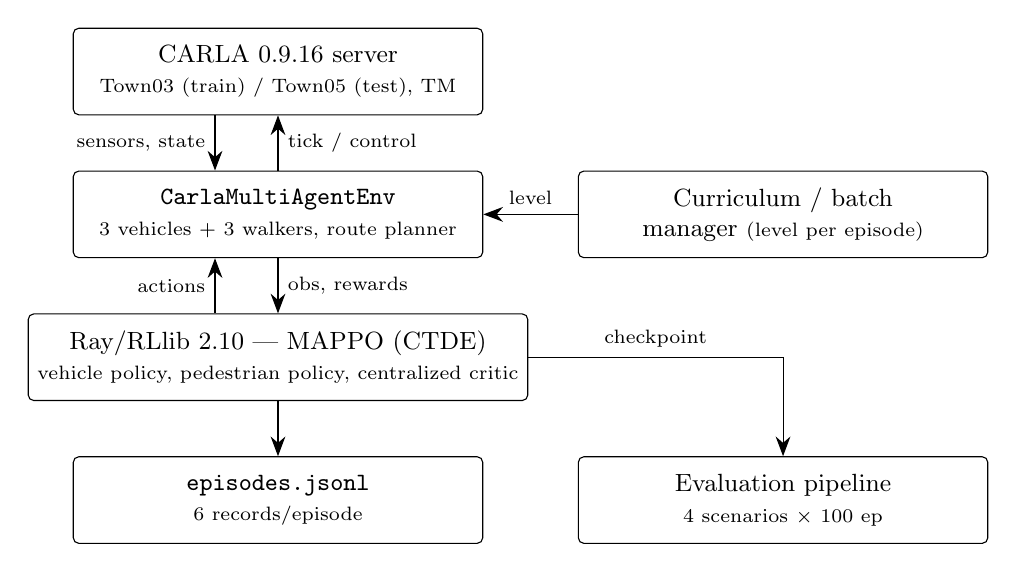
\begin{tikzpicture}[
      node distance=7mm and 12mm,
      box/.style={draw, rounded corners=2pt, align=center,
                  minimum width=52mm, minimum height=11mm, font=\small},
      lbl/.style={font=\scriptsize, midway},
      >={Stealth[length=2.5mm]}]
    \node[box] (carla) {CARLA 0.9.16 server\\ \scriptsize Town03 (train) / Town05 (test), TM};
    \node[box, below=of carla] (env) {\texttt{CarlaMultiAgentEnv}\\ \scriptsize 3 vehicles + 3 walkers, route planner};
    \node[box, right=of env] (mgr) {Curriculum / batch\\ manager \scriptsize (level per episode)};
    \node[box, below=of env] (rllib) {Ray/RLlib 2.10 --- MAPPO (CTDE)\\ \scriptsize vehicle policy, pedestrian policy, centralized critic};
    \node[box, below=of rllib] (log) {\texttt{episodes.jsonl}\\ \scriptsize 6 records/episode};
    \node[box, right=of log] (eval) {Evaluation pipeline\\ \scriptsize $4$ scenarios $\times$ 100 ep};
    \draw[->] (env) -- node[lbl, right] {tick / control} (carla);
    \draw[<-] ([xshift=-8mm]env.north) -- node[lbl, left] {sensors, state} ([xshift=-8mm]carla.south);
    \draw[->] (mgr) -- node[lbl, above] {level} (env);
    \draw[->] (env) -- node[lbl, right] {obs, rewards} (rllib);
    \draw[<-] ([xshift=-8mm]env.south) -- node[lbl, left] {actions} ([xshift=-8mm]rllib.north);
    \draw[->] (rllib) -- (log);
    \draw[->] (rllib) -| node[lbl, above, pos=0.25] {checkpoint} (eval);
  \end{tikzpicture}
  \caption{Component architecture. The curriculum/batch manager is the only
  component that differs between the two experimental arms, and only in its
  level-selection rule (\cref{sec:regimes}).}
  \label{fig:architecture}
\end{figure}

% ------------------------------------------------------------
\section{A Shared-World Multi-Agent Environment}
\label{sec:shared-world}

\subsection{Parallel task coverage}
\label{sec:parallel-coverage}

The six learning agents do not cooperate toward a joint goal: each agent is
assigned its \emph{own} route and is evaluated individually on completing
it. Because all six routes are placed in the same living world, a single
episode simultaneously exercises six different micro-tasks --- different
road geometries, different interactions with scripted traffic, and, most
importantly, mutual interactions between learning agents (e.g.\ a learning
vehicle yielding to a learning pedestrian). We refer to this design as
\emph{parallel task coverage}: per wall-clock episode, the system collects
experience across six task instances rather than one.

This framing comes with two caveats that the analysis must respect. First,
the six per-episode samples are \emph{correlated} --- the agents share the
world state, so a traffic jam or a blocked crosswalk affects several
records at once. Second, from the perspective of any single agent the
environment is \emph{non-stationary} during training, because the other
five agents' policies change over time; this is the standard motivation for
the CTDE critic (\cref{ch:background}). Parallel task coverage is a
property of the platform, present identically in both training regimes: it
is part of the experimental frame, not an experimental variable.

\subsection{Per-agent routes and seeding}
\label{sec:seeding}

At every reset, each agent receives an independent route whose target
length is set by the active difficulty level (30/60/\SI{100}{m};
\cref{sec:routes}). Route generation is deterministically seeded per agent
with a seed sequence built from
$\langle\text{traffic seed},\ \text{reset counter},\ \mathrm{crc32}(\text{agent
id})\rangle$, so that (i) two training runs launched with the same
experiment seed on the same code see the same sequence of route-generation
draws, and (ii) route draws are decoupled across agents. This makes paired
A/B comparisons route-matched by construction, a property the experimental
protocol relies on (\cref{ch:methodology}).

\subsection{Termination taxonomy and per-agent records}
\label{sec:termination}

Each agent terminates its episode independently with exactly one of six
reasons, classified by a simulator-independent rule
(\texttt{episode\_classification.py}):

\begin{itemize}
  \item \texttt{route\_complete} --- the agent reached the end of its
        route. This is the \emph{only} outcome counted as success.
  \item \texttt{route\_short} --- the agent reached the end of a route
        whose optimal length turned out to be shorter than the level target
        by more than a tolerance factor (degenerate route-generation
        fallback). Reaching it is \emph{not} counted as success: this guard
        prevents success-rate inflation through trivially short routes.
  \item \texttt{collision} --- contact with any actor or static geometry.
  \item \texttt{offroad} --- the vehicle moved more than \SI{5}{m} away
        from the nearest driving-lane centre (vehicles only).
  \item \texttt{stuck} --- prolonged lack of progress along the route.
  \item \texttt{timeout} --- the 1{,}000-step episode cap elapsed first.
\end{itemize}

Every episode therefore yields exactly six agent-level records (three
vehicle, three pedestrian) in \texttt{episodes.jsonl}. All aggregate
metrics in this thesis are computed at the agent level over these records,
always reported separately for vehicles and pedestrians; the measurement
rules, including deduplication and the strict success criterion, are
specified in \cref{ch:methodology}.

% ------------------------------------------------------------
% Sources (verified 2026-07-14): carla_multi_agent_env.py
%   _get_vehicle_obs L1291-1381, _get_pedestrian_obs L1383-1445,
%   _fill_nearby L1740-1764, constants L84-88; global obs layout
%   centralized_critic.py (compute_global_obs_dim_with_mask, L115).
\section{Observation and Action Spaces}
\label{sec:obs-actions}

Each agent receives a compact, class-specific observation vector with all
components normalized to $[-1, 1]$ and sanitized against non-finite values
before being returned to the learner. Vehicles observe 47 dimensions and
pedestrians 26; \cref{tab:obs} lists both layouts. Three design choices
deserve comment.

\paragraph{Route-aware features.}
Beyond the classic ego-kinematics and nearest-neighbour features, both
classes observe a short \emph{preview} of their own route (relative
offsets of upcoming waypoints in the ego frame) together with heading
error and, for vehicles, upcoming turn angle and signed lateral error.
These features give the policy the local geometry of the assigned task
without revealing anything about the other agents' goals.

\paragraph{Hazard preview channel.}
A shared routine estimates, along the agent's forward corridor, a
time-to-collision risk and a corridor-occupancy fraction, computed
separately against vehicles (corridor \SI{3.5}{m} wide, \SI{40}{m} ahead,
\SI{5}{s} horizon) and against pedestrians (\SI{3.0}{m}, \SI{30}{m},
\SI{4}{s}); pedestrians observe the vehicle channel only (\SI{4.0}{m},
\SI{30}{m}, \SI{4}{s}). The same four vehicle-side risk values are reused
by the reward function as a safety gate (\cref{sec:rewards}), so the
quantity that modulates the reward is always visible to the policy.

\paragraph{Markov-consistency features.}
The last three vehicle dimensions expose internal environment state that
the reward depends on: the number of steps without waypoint progress
(normalized by 300), the state of the anti-loop penalty, and the
normalized time remaining before episode truncation. Without these, the
penalties of \cref{sec:rewards} and the fixed horizon would act on
information the agent cannot observe --- a state-aliasing defect that was
identified and corrected during development (\cref{ch:methodology}).

\begin{table}[t]
  \centering\small
  \caption{Observation layouts. Slashes denote normalization constants;
  neighbour features are expressed in the ego frame.}
  \label{tab:obs}
  \begin{tabular}{@{}llp{8.0cm}@{}}
    \toprule
    Dims & Group & Content \\
    \midrule
    \multicolumn{3}{@{}l}{\emph{Vehicle (47D)}} \\
    0--8   & Ego kinematics   & velocity (/30), acceleration (/10), speed (/120 km/h), planar heading \\
    9--12  & Route tracking   & distance (/\SI{50}{m}) and bearing (/$\pi$) to next waypoint; signed in-lane lateral offset (lane widths); continuous route progress \\
    13--14 & Traffic light    & at-light flag; state (red 1.0, yellow 0.5, green 0.0) \\
    15--23 & Nearby vehicles  & 3 nearest within \SI{50}{m}: longitudinal and lateral offset (/50), relative speed (/30) \\
    24     & Control memory   & previous steering command \\
    25--30 & Route preview    & waypoints $+1/+3/+5$: longitudinal and lateral offsets (/50) \\
    31--33 & Route geometry   & heading error; upcoming turn angle; signed lateral error to route \\
    34--39 & Nearby pedestrians & 2 nearest within \SI{50}{m}, same 3 features \\
    40--43 & Hazard preview   & time-to-collision risk and corridor occupancy, vs.\ vehicles and vs.\ pedestrians \\
    44--46 & Progress/time    & steps without progress (/300); loop-penalty flag; time remaining \\
    \midrule
    \multicolumn{3}{@{}l}{\emph{Pedestrian (26D)}} \\
    0--2   & Position         & world position ($x, y$ /500; $z$ /50) \\
    3--6   & Kinematics       & velocity (/5), speed (/5 m/s) \\
    7--8   & Heading          & planar forward vector \\
    9--10  & Waypoint         & distance (/\SI{100}{m}) and bearing to current waypoint \\
    11     & Surface          & on-sidewalk flag \\
    12--17 & Nearby vehicles  & 2 nearest within \SI{50}{m}: same 3 features \\
    18     & Progress         & route completion fraction \\
    19--22 & Route preview    & waypoints $+1/+3$: longitudinal and lateral offsets (/100) \\
    23     & Route geometry   & heading error \\
    24--25 & Hazard preview   & vehicle time-to-collision risk and corridor occupancy \\
    \bottomrule
  \end{tabular}
\end{table}

\paragraph{Action spaces.}
Both classes use continuous two-dimensional actions. The vehicle action is
$[a_{\mathrm{tb}}, a_{\mathrm{steer}}] \in [-1,1]^2$, where positive
$a_{\mathrm{tb}}$ maps to throttle and negative to brake (reverse gear is
disabled), and $a_{\mathrm{steer}}$ is the steering command. The
pedestrian action is $[a_{\mathrm{speed}}, a_{\Delta\mathrm{h}}]$ with
$a_{\mathrm{speed}} \in [0,1]$ scaling a maximum walking speed of
\SI{5.0}{m/s} and $a_{\Delta\mathrm{h}} \in [-1,1]$ commanding a heading
change of up to $\pm 45^{\circ}$ per step.

\paragraph{Global observation for the centralized critic.}
During training only, the critic receives a fixed-slot concatenation of
all agents' observations followed by a per-agent alive mask:
$[\,v_0\,|\,v_1\,|\,v_2\,|\,p_0\,|\,p_1\,|\,p_2\,|\,\text{alive}_{6}\,]$,
i.e.\ $3 \times 47 + 3 \times 26 + 6 = 225$ dimensions. The alive mask is
necessary because agents terminate independently
(\cref{sec:termination}): slots of terminated agents are masked rather
than silently reused. Actors never see this vector, preserving
decentralized execution.

% ------------------------------------------------------------
% Sources (verified 2026-07-14): carla_multi_agent_env.py
%   _vehicle_reward L1866-1960 ("Vehicle Reward v5"),
%   _pedestrian_reward L1962-2010 ("Pedestrian Reward v5").
\section{Reward Design}
\label{sec:rewards}

Rewards are per-agent and identical in both training regimes.
\Cref{tab:rewards} lists every component with its trigger and magnitude;
this section explains the structure. The final form is the outcome of the
gate-driven iterations documented in \cref{sec:iterations}; no claim of
optimality is attached to the individual coefficients.

\paragraph{Progress core.}
For both classes the dominant signal is a sparse bonus per route waypoint
reached ($+100$ for vehicles, $+50$ for pedestrians), complemented by a
dense shaping term proportional to the per-step reduction of the distance
to the next waypoint. Waypoints skipped by cutting across the route are
penalized, so progress cannot be gamed by shortcuts.

\paragraph{Safety terms.}
A collision costs vehicles $-500$, applied once at the step of first
contact (the episode then terminates). Two further vehicle terms penalize
leaving the lane (linear beyond \SI{2}{m} from the lane centre; episode
termination occurs at \SI{5}{m}, \cref{sec:termination}) and exceeding
50~km/h. Pedestrian collisions cost $-50$, and pedestrians receive a
small per-step incentive to stay on sidewalks rather than on driving
lanes.

\paragraph{Hazard-gated anti-stall shaping (vehicles).}
The empirically most delicate block counteracts the \emph{defensive
equilibrium} in which a vehicle stops indefinitely to avoid any risk. All
of its terms are suspended while the vehicle is legitimately waiting at a
red or yellow light. The scalar $\mathit{hazard} =
\max(\text{TTC}_{\mathrm{veh}}, \text{occ}_{\mathrm{veh}},
\text{TTC}_{\mathrm{ped}}, \text{occ}_{\mathrm{ped}})$ summarizes the
hazard-preview channel of \cref{sec:obs-actions}, and a boolean
$\mathit{safe\_to\_push} = (\mathit{hazard} < 0.85)$ gates the pushing
terms: an idle penalty below 2.5~km/h; a start bonus proportional to
throttle, route alignment, and an urgency factor that grows with the time
spent without progress; and a minimum-speed shaping around a target of
8~km/h, active only when the vehicle is aligned with its route (alignment
$> 0.25$). Above the hazard threshold every pushing incentive disappears,
so the policy is never rewarded for accelerating into a risky corridor.
Independently of the gate, a no-progress ramp (after 100 steps without
reaching a waypoint) and an anti-loop penalty make prolonged stalling and
circling strictly unprofitable, and a steering-smoothness pair discourages
jerky control.

\paragraph{Pedestrian pace band.}
Pedestrians earn a per-step bonus while walking within a comfort band of
$[1.2, 2.6]$~m/s, with an idle penalty below 0.15~m/s and a running
penalty above 3.0~m/s. The band is intentionally wide: at 2.0~m/s a
pedestrian covers \SI{100}{m} --- the hard-level target --- within the
\SI{50}{s} horizon. The bonus-only (asymmetric) design of this band and
its interaction with the vehicles' hazard gate are analysed empirically in
\cref{ch:results}.

\begin{table}[t]
  \centering\small
  \caption{Reward components. ``Gated'' vehicle rows are suspended while
  waiting at a red/yellow light; rows marked $^{\dagger}$ additionally
  require $\mathit{safe\_to\_push}$ ($\mathit{hazard} < 0.85$) and route
  alignment $> 0.25$.}
  \label{tab:rewards}
  \begin{tabular}{@{}p{3.4cm}p{5.6cm}p{4.6cm}@{}}
    \toprule
    Component & Trigger & Value \\
    \midrule
    \multicolumn{3}{@{}l}{\emph{Vehicle}} \\
    Waypoint reached      & per waypoint advanced & $+100$ \\
    Skipped waypoint      & per waypoint skipped & $-10$ \\
    Dense progress        & change in distance to next waypoint & $+4.0$ per metre closed \\
    Collision             & first contact (terminal) & $-500$ \\
    Off-lane              & $>$ \SI{2}{m} from lane centre & $-0.5$ per metre \\
    Overspeed             & speed $> 50$ km/h & $-0.10$ per km/h over \\
    Idle (gated)          & speed $< 2.5$ km/h & $-0.15$ \\
    Start bonus (gated$^{\dagger}$) & throttle while idle & $(0.20 + 0.30\,u)\cdot\text{thr}\cdot\text{align}$, brake symmetric; $u = \min(\text{no-progress}/200, 1)$ \\
    Min-speed shaping (gated$^{\dagger}$) & speed below / above 8 km/h & $-0.04\,(8 - v)\cdot\text{align}$ / $+0.15\cdot\text{align}$ \\
    No-progress ramp (gated) & $>$ 100 steps without waypoint & $-0.004$ per step, capped $-1.0$ \\
    Smooth steering       & $|\Delta \text{steer}| < 0.1$ at $> 5$ km/h & $+0.1$ \\
    Steering jerk         & $|\Delta \text{steer}| > 0.5$ & $-0.3$ \\
    Anti-loop             & loop detector active & $-1.0$ \\
    \midrule
    \multicolumn{3}{@{}l}{\emph{Pedestrian}} \\
    Waypoint reached      & per waypoint advanced & $+50$ \\
    Skipped waypoint      & per waypoint skipped & $-10$ \\
    Dense progress        & change in distance to waypoint & $+2.0$ per metre closed \\
    Collision             & first contact (terminal) & $-50$ \\
    Sidewalk / roadway    & per step on sidewalk / driving lane & $+0.2$ / $-0.3$ \\
    Walking pace          & speed $\in [1.2, 2.6]$ m/s & $+0.3$ \\
    Idle                  & speed $< 0.15$ m/s & $-0.15$ \\
    Running               & speed $> 3.0$ m/s & $-0.7$ per m/s over \\
    Anti-loop             & loop detector active & $-1.0$ \\
    \bottomrule
  \end{tabular}
\end{table}

% ------------------------------------------------------------
% Sources (verified 2026-07-14): route_planner.py (min_route_ratio=0.5,
%   max_route_ratio=2.0 L145-146/206-207, max_cross=3 L261/329, short-chain
%   rejection L368-369); levels.yaml (levels_path 30/60/100, test Town05 80);
%   route_source labels carla_multi_agent_env.py L1040-1159.
\section{Route Generation and Difficulty Levels}
\label{sec:routes}

Difficulty is defined by the \emph{target length} of the per-agent routes,
with all other scenario parameters held constant: the three training
levels (easy, medium, hard) place both vehicle and pedestrian targets at
30, 60 and \SI{100}{m} respectively, always on Town03 and always with the
same scripted traffic (15 NPC vehicles, 30 NPC pedestrians). A fourth,
evaluation-only level (\emph{test}) uses Town05 with \SI{80}{m} targets
and the same traffic counts. The configuration also defines level families
where difficulty varies by traffic density instead of route length; these
are not used in this thesis (\cref{sec:campaign}).

\paragraph{Vehicle routes.}
Vehicle routes are planned on the road topology with CARLA's global route
planner: candidate destinations are sampled around the target distance and
a candidate is accepted only if its optimal path length lies within
$[0.5, 2.0] \times$ the target, with up to 32 attempts per reset. If no
candidate survives, the environment falls back to a legacy waypoint-chain
generator. The applied generator is recorded per record
(\texttt{route\_source} $\in$ \{\texttt{grp},
\texttt{legacy\_fallback}\}), so the share of fallback routes is always
measurable.

\paragraph{Pedestrian routes.}
Pedestrian routes are chains of sidewalk segments connected through
crosswalks. Two constraints shape them: chains whose cumulative length
falls below $0.5 \times$ the target are rejected (the same lower-bound
guard that backs the \texttt{route\_short} demotion of
\cref{sec:termination}), and the number of crosswalk crossings per route
is capped at three --- a bound on the pedestrians' on-roadway exposure
whose value was set empirically (\cref{sec:iterations}). The generator
records its outcome per record (\texttt{sidewalk\_crosswalk},
\texttt{sidewalk\_distance}, \texttt{respawn}, \texttt{legacy\_chain}),
together with feasibility diagnostics (optimal length, target error,
under-target and too-short flags, candidate attempts). Pedestrian route
feasibility on Town03 is a structural limitation of the platform ---
sidewalk topology often cannot support the nominal medium/hard targets ---
and is analysed separately in \cref{sec:ped-limits}, where environment
limits are explicitly distinguished from policy limits.

\todo{Fig.~3: example routes per level. Generator script ready at
\texttt{docs/thesis/scripts/make\_fig3\_route\_examples.py} (requires a
live CARLA server; user runs it); then include
\texttt{figures/route\_examples.pdf} here.}

% ------------------------------------------------------------
% Sources (verified 2026-07-14): curriculum_batch.yaml (all thresholds);
%   curriculum_batch_manager.py (_balanced_policy_success_details L391-423:
%   min over policies; window_full L129/382; BatchLevelSampler L902-940).
\section{Curriculum and Mixed-Batch Training Regimes}
\label{sec:regimes}

The training regime is the independent variable of the main experiment.
Both regimes are implemented by the same manager component, consulted once
per episode reset to select the difficulty level; they share the level
definitions of \cref{sec:routes}, the total budget of $3 \times 10^6$
environment steps, and every other component described in this chapter.
They differ \emph{only} in the level-selection rule.

\subsection{Curriculum arm: competence-gated progression}
\label{sec:curriculum-arm}

Training starts with only the easy level unlocked. Higher levels unlock
through a competence gate evaluated on a sliding window of the last 50
episodes: the windowed success rate is computed separately for the vehicle
policy and the pedestrian policy, and the gate binds on the \emph{minimum}
of the two --- progression requires the weaker class to be competent, not
the average. Medium unlocks at a windowed success rate of at least 70\%,
hard at 60\%; the window must be full, and a minimum share of the total
budget must already have been spent at the preceding levels (20\% on easy
before medium; 28\% on medium before hard). Two design decisions deserve
justification:

\begin{itemize}
  \item \textbf{Windowed, not cumulative.} The cumulative success rate is
        a lagging integrator dragged down by cold-start failures: a policy
        can be competent \emph{now} while its since-birth average is still
        far below threshold. Gating on a sliding window measures current
        competence.
  \item \textbf{Pressure caps.} If a threshold is never met, the level
        force-unlocks anyway once a fixed share of the total budget has
        been consumed (30\% for medium, 70\% for hard). This guarantees
        that every level is visited within the budget, so the curriculum
        arm can never terminally stall on easy --- at worst it degrades
        toward a delayed mixed exposure.
\end{itemize}

Once unlocked, levels are sampled with weights that normalize to
$0.30/0.35/0.35$ (easy/medium/hard) under budget constraints (easy at most
30\% of the budget once medium is available, medium at most 35\%, hard at
least 35\%). Newly unlocked levels pass through a short \emph{probation}
phase with reduced sampling pressure (hard is temporarily de-emphasized at
weight 0.85), smoothing the transition instead of switching abruptly.

\subsection{Batch arm: stratified interleaving}
\label{sec:batch-arm}

The mixed-batch arm is the \emph{no-ordering control}: all three levels
are available from the first episode. Levels are sampled by stratified
shuffling without replacement with a window of three: each consecutive
window of three episodes drawn from one sampler instance is a uniformly
random permutation of \{easy, medium, hard\}, giving uniform $1/3$
exposure with a maximum imbalance of one episode per sampler --- avoiding
both the drift of i.i.d.\ sampling and any fixed deterministic ordering
within the window. In the realized campaign logs, where episodes from
parallel rollout workers interleave, the global level shares stay within
$\approx 2$ percentage points of uniform and all three levels appear
within the first twenty episodes (\cref{sec:integrity}).

\subsection{What the comparison isolates}
\label{sec:isolation}

Under this construction, the two arms consume the same budget over the
same task distribution in expectation; what differs is \emph{when} each
part of that distribution is presented and whether presentation is
conditioned on measured competence. Any behavioural difference between the
arms is therefore attributable to the ordering policy, up to run-to-run
variance --- which is quantified separately in \cref{ch:results} and
discussed in \cref{sec:threats}.

\begin{figure}[t]
  \centering
  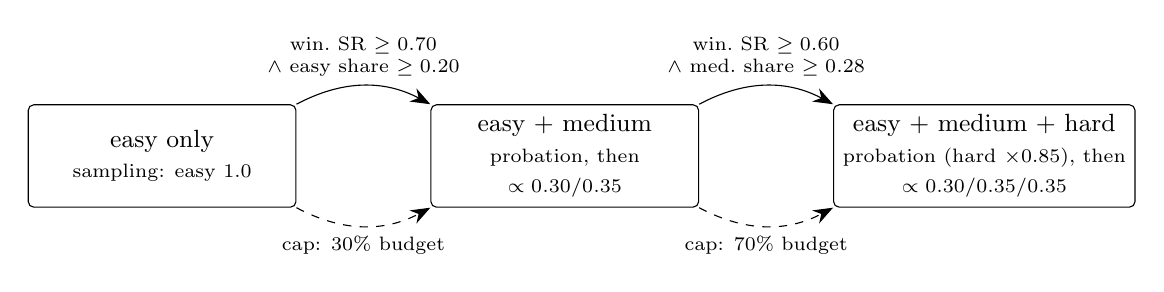
\begin{tikzpicture}[
      state/.style={draw, rounded corners=2pt, align=center,
                    minimum width=34mm, minimum height=13mm, font=\small},
      gate/.style={font=\scriptsize, align=center},
      >={Stealth[length=2.5mm]}, node distance=17mm]
    \node[state] (s1) {easy only\\ \scriptsize sampling: easy 1.0};
    \node[state, right=of s1] (s2) {easy $+$ medium\\ \scriptsize probation, then\\ \scriptsize $\propto 0.30/0.35$};
    \node[state, right=of s2] (s3) {easy $+$ medium $+$ hard\\ \scriptsize probation (hard $\times$0.85), then\\ \scriptsize $\propto 0.30/0.35/0.35$};
    \draw[->] (s1.north east) to[bend left=28]
      node[gate, above] {win.\ SR $\geq 0.70$\\ $\wedge$ easy share $\geq 0.20$} (s2.north west);
    \draw[->, dashed] (s1.south east) to[bend right=28]
      node[gate, below] {cap: 30\% budget} (s2.south west);
    \draw[->] (s2.north east) to[bend left=28]
      node[gate, above] {win.\ SR $\geq 0.60$\\ $\wedge$ med.\ share $\geq 0.28$} (s3.north west);
    \draw[->, dashed] (s2.south east) to[bend right=28]
      node[gate, below] {cap: 70\% budget} (s3.south west);
  \end{tikzpicture}
  \caption{Curriculum progression. Solid edges: competence gates on the
  windowed success rate (minimum over the two policies, window of 50
  episodes, window full) with budget-share floors. Dashed edges: pressure
  caps guaranteeing progression within the budget. In the campaign's
  MLP-curriculum run (seed 999), medium unlocked at episode 842 of 3{,}220
  (26.1\%) and hard at episode 2{,}286 (71.0\%), for a final level mix of
  32.5\% easy / 45.8\% medium / 21.6\% hard --- timings consistent with
  the pre-campaign trunk replicates.}
  \label{fig:curriculum-fsm}
\end{figure}

% ------------------------------------------------------------
% Sources (verified 2026-07-14): centralized_critic.py (GraphConvLayer
%   L336-356, GNNCriticEncoder L414-497, critic MLP 225->256->256->1);
%   run_config.json of campaign runs (all optimizer values, byte-identical
%   across arms except mode/use_gnn).
\section{Critic Encoder Variants and Training Pipeline}
\label{sec:critic-variants}

\subsection{Critic encoders}
\label{sec:critic-encoders}

In the default configuration the centralized critic is an MLP mapping the
225-dimensional global observation through two hidden layers of 256 units
to a scalar value. The secondary experimental axis
(\cref{sec:campaign}) replaces this encoder with a graph-based one, while
\emph{both actors remain the identical MLPs} of \cref{sec:architecture}:
any behavioural difference between the two variants is therefore
attributable to value estimation during training, not to policy capacity,
and at execution time the two variants are indistinguishable in
architecture.

The GNN encoder splits the global observation back into the six per-agent
slots, projects each through a per-class linear layer into a
64-dimensional node embedding, and applies two rounds of message passing
with GraphSAGE-style mean aggregation~\cite{hamilton2017graphsage}: each
node combines its own embedding with the mean of the other \emph{alive}
agents' embeddings through separate learned weights, followed by an ELU
activation. A masked mean-pool over alive nodes produces the input to the
value head. The alive mask from the global observation drives both the
aggregation and the pooling, so terminated agents drop out of the
critic's summary instead of contributing stale slots. (The codebase also
provides an attention-based critic encoder and PopArt value
normalization behind configuration flags; both remain disabled throughout
this thesis.)

\subsection{Optimization settings}
\label{sec:optimization}

All campaign runs share the same optimizer configuration, byte-identical
across arms except for the regime and encoder flags: learning rate
$5\times10^{-4}$; discount $\gamma = 0.997$; GAE $\lambda = 0.95$; PPO
clip 0.2 with an additional KL penalty (target 0.02); gradient clipping at
0.5; value-loss coefficient 0.05 with the value clip effectively disabled
($10^6$); training batch 8{,}000 steps, minibatch 256, 15 SGD epochs per
batch, rollout fragments of 200 steps. The entropy coefficient follows a
schedule from 0.03 to 0.005 with the transition anchored at 83\% of the
total budget (step 2.49M of 3M) --- expressed as a budget fraction so that
short diagnostic runs and full runs traverse the same exploration profile.
The full configuration files are reproduced in \cref{app:hyperparams};
the empirical justification of the non-default values (notably $\gamma$,
the value-loss settings, and the entropy schedule) is part of the
iterative record in \cref{ch:methodology}.

\subsection{Evaluation pipeline}
\label{sec:eval-pipeline}

Results are measured at three levels, all computed from agent-level
records (\cref{sec:termination}):

\begin{enumerate}
  \item \textbf{Training stream}: the cumulative metrics over all training
        episodes. These are on-policy and, in the curriculum arm, computed
        over a level mix that changes over time --- they characterize the
        training process, not final ability.
  \item \textbf{Static recomputation}: an offline pass over the training
        logs that recomputes all aggregates from disk, deduplicates
        records, and verifies integrity (exactly six records per episode,
        no non-finite values).
  \item \textbf{Final checkpoint evaluation}: the trained checkpoint is
        reloaded and run on four fixed scenarios of 100 episodes each ---
        easy, medium and hard on Town03, plus the test level on Town05
        (\cref{sec:routes}), the latter measuring map generalization on
        roads never seen in training. Episodes are evaluated with the
        stochastic policy (sampling from the learned Gaussian) and
        per-episode reseeding of both the scenario and the action sampler.
        Evaluating the deterministic policy mean was deliberately
        rejected: for a continuous Gaussian policy it collapses behaviour
        onto a single trajectory per scenario, a failure mode analysed in
        \cref{sec:bugs}.
\end{enumerate}

% ============================================================
% Chapter 4 — Experimental Methodology (target 8–9 pp)
% Status: FULL DRAFT 2026-07-14.
% Sources: CLAUDE.md <measurement_rules>/<gate_policy>/<experimental_state>
%   (repo-tracked project record), docs/EXPERIMENT_REGISTRY.md (App. A),
%   episode_classification.py L69-85 (stuck/timeout split),
%   carla_multi_agent_env.py L522-565 (path_efficiency).
% All development-phase numbers below are quoted from the project registry
% and are tied to run IDs; per-candidate detail condensed in Appendix A.
% ============================================================
\chapter{Experimental Methodology}
\label{ch:methodology}

The platform of \cref{ch:system} was not designed in one pass: it is the
product of an iterative campaign in which every change had to pass a
predefined quantitative gate before entering the trunk. This chapter
documents the measurement rules (\cref{sec:metrics}), the gate protocol
(\cref{sec:gate}), the validity defects found and fixed along the way
(\cref{sec:bugs}), a summary of the iterations themselves
(\cref{sec:iterations}), and the design of the final comparison campaign
(\cref{sec:campaign}).

% ------------------------------------------------------------
\section{Metrics and Measurement Rules}
\label{sec:metrics}

\paragraph{Unit of measurement.}
The unit of analysis is the \emph{agent-level record}: one JSON entry per
agent per episode (six per episode, \cref{sec:termination}). All
aggregates are computed over records after deduplication by episode and
agent identifier (in evaluation, the scenario is part of the key, since
episode identifiers can repeat across scenarios). Two integrity conditions
are enforced before any number is reported: exactly six records per
episode, and no non-finite value in any field. A run failing either
condition is not analysed further.

\paragraph{Strict success criterion.}
An agent is successful if and only if its termination reason is
\texttt{route\_complete}. In particular, \texttt{route\_short} --- reaching
the end of a degenerately short route --- is \emph{not} success
(\cref{sec:termination}). This rule was stress-tested during development:
a change that counted \texttt{route\_short} as success was introduced and
subsequently reverted (\cref{sec:iterations}), keeping the criterion
strict at the cost of lower absolute numbers. \Cref{ch:discussion}
discusses why mid-range absolute success rates are a feature, not a
defect, of the resulting measurement: away from floor and ceiling, the
metric retains room to move in both directions, which is precisely what a
comparative study needs.

\paragraph{Three reporting views.}
Every result is reported for vehicles and pedestrians separately, plus a
combined view; the two classes have different tasks, different action
spaces and different structural limits (\cref{sec:ped-limits}), and the
experimental record shows regime effects that exist for one class only.
Joint episode-level success (``all six agents succeed'') is never used:
with correlated agents in a shared world it compounds failures
multiplicatively and hides class-specific structure.

\paragraph{Metric catalogue.}
\Cref{tab:metrics} defines the metrics used throughout
\cref{ch:results}. Cumulative values over all training episodes are the
primary aggregation; sliding-window success (window 50) is used only by
the curriculum gate (\cref{sec:regimes}); within-run dynamics are shown
by splitting training into quartiles (Q1--Q4).

\begin{table}[t]
  \centering\small
  \caption{Metric catalogue. All rates are shares of agent-level records.}
  \label{tab:metrics}
  \begin{tabular}{@{}p{3.6cm}p{9.6cm}@{}}
    \toprule
    Metric & Definition \\
    \midrule
    Success rate (SR) & records with \texttt{route\_complete} \\
    Collision rate & records with \texttt{collision} \\
    Offroad rate & records with \texttt{offroad} (vehicles) \\
    Stuck rate & truncated records with route completion $< 0.3$ or an active loop detector \\
    Timeout rate & truncated records with route completion $\geq 0.3$ \\
    Stuck$+$timeout & sum of the previous two; the primary anti-stall target \\
    Route completion & fraction of route waypoints consumed, $[0,1]$ \\
    Path efficiency & completed optimal length / actual distance travelled, capped at 1; defined as 0 for stuck records \\
    Mean speed & km/h for vehicles, m/s for pedestrians \\
    No-progress steps & steps since the last waypoint advance, at episode end \\
    Route diagnostics & \texttt{route\_source} shares, under-target and too-short flags, crossing counts (\cref{sec:routes}) \\
    \bottomrule
  \end{tabular}
\end{table}

% ------------------------------------------------------------
\section{Gate-Driven Development Protocol}
\label{sec:gate}

Run-to-run variance in this environment is large (quantified below at
$\sim$10 percentage points of vehicle SR between identical replicates),
and the available compute budget did not allow replicating every candidate
change. The protocol adopted in response has four rules.

\paragraph{1. One knob at a time.}
Every candidate is a narrow, behaviourally isolated diff --- a single
reward term, a single threshold, a single observation group. Candidates
touching the same file are evaluated sequentially, never stacked. When a
bundled change failed its gate, attribution between its halves was treated
as unresolved rather than guessed.

\paragraph{2. Paired A/B at a fixed diagnostic budget.}
Each candidate runs for $3\times10^{5}$ steps against the current trunk
baseline, with the same experiment seed and, thanks to the deterministic
route seeding of \cref{sec:seeding}, a route sequence paired with the
baseline by construction. Development-phase runs were locked to the easy
level unless the candidate targeted the curriculum itself, so that level
mixing could not confound the comparison. When runs of different lengths
are compared, records are truncated to equal episode counts.

\paragraph{3. A predefined quantitative gate.}
For vehicle-focused changes the candidate is promoted only if, versus the
paired baseline: vehicle SR improves by at least $+2.0$\,pp;
stuck$+$timeout improves by at least $-2.0$\,pp; collision and offroad
each worsen by no more than $+1.0$\,pp; and both integrity conditions of
\cref{sec:metrics} hold. Changes that touch shared machinery carry a
\emph{must-not-collapse} side condition on the other class (pedestrian SR
within $-2$\,pp). A failed gate means the candidate is reverted; the trunk
is never left in a partially evaluated state.

\paragraph{4. Mechanism and outcome are recorded separately.}
For each candidate the registry records whether the intended
\emph{mechanism} occurred (e.g.\ the critic's explained variance rising
from $\approx 0$ to $0.87$ after a value-loss fix) and whether the
\emph{behavioural gate} passed --- the two frequently dissent. A small
number of gate-failing knobs were knowingly retained with the hypothesis
recorded as falsified (e.g.\ a tenfold collision penalty that left the
collision rate flat), because reverting them would have restored a defect
or because the failure itself was informative. These exceptions are
explicit in the registry (\cref{app:registry}); nothing was retained
silently.

Within-run quartile trajectories complement the gate: a candidate whose
cumulative numbers pass but whose Q4 declines (a signature observed for
one pedestrian-pace retune) is treated as rejected.

% ------------------------------------------------------------
\section{Environment Validity: Bugs Found and Fixed}
\label{sec:bugs}

In a custom multi-agent platform the measurement apparatus is part of the
experiment. Three episodes during development produced apparent policy
effects that were in fact artifacts; they are reported here both because
they shaped the final protocol and because their detection signatures may
be useful to others.

\paragraph{Route-length bug (task distribution).}
The route planner could emit routes far longer than the level target, so
nominal ``easy'' episodes were frequently not easy. Enforcing the
$[0.5, 2.0]\times$ target bounds (\cref{sec:routes}) moved cumulative
vehicle training SR by $\approx +50$\,pp \emph{with no change to the
policy or the reward} --- a pure task-distribution change. Two
consequences were adopted: absolute metrics are only comparable within the
same environment version, and all earlier results were re-labelled as
era-specific (the vehicle floor of the April pilot,
\cref{sec:pilot}, was later traced to this defect). This episode is the
strongest internal evidence for a rule used throughout this thesis:
\emph{never compare absolute numbers across environment versions; anchor
claims to paired contrasts within a version}.

\paragraph{Route-seeding bug (broken pairing).}
Per-agent route seeds were originally derived from Python's built-in
\texttt{hash()}, which is salted per process: two nominally identical runs
drew \emph{different} route sequences, silently degrading every A/B
comparison. The fix derives seeds from an explicit
\texttt{SeedSequence} over traffic seed, reset counter and a stable digest
of the agent identifier (\cref{sec:seeding}). The lesson: pairing must be
constructed and verified (byte-identical route-generation statistics
across arms), not assumed.

\paragraph{Evaluation-pipeline bugs (measurement collapse).}
The first checkpoint evaluation returned a success rate of exactly
33.33\% in every scenario --- one of three vehicles completing, every
episode. This ``too clean to be true'' pattern exposed four coupled
defects: (i) the per-episode scenario seed was constant, so every episode
replayed the same traffic configuration; (ii) the policy was evaluated at
its deterministic mean, collapsing the Gaussian policy onto a single
trajectory per scenario; (iii) the evaluation subprocess never initialized
the episode logger, so no agent-level records were written at all; and
(iv) the torch seed was constant across episode subprocesses, so even
stochastic actions would have replayed correlated noise streams. All four
were fixed (per-episode scenario and sampler seeds, stochastic
evaluation, logger propagation with clean restart), the partial
deterministic evaluation was discarded, and the stochastic protocol of
\cref{sec:eval-pipeline} became the standard. None of these fixes touches
training; per the project's own rules, no policy claim is derived from
them.

The general lesson of this section: measurement validity has to be
established \emph{before} tuning, and implausibly regular results are a
detection signal, not good news.

% ------------------------------------------------------------
\section{Iterative Development Summary}
\label{sec:iterations}

\Cref{tab:candidates} condenses the development record; the full
per-candidate registry, with run IDs and mechanisms, is in
\cref{app:registry}. Development proceeded in six phases:

\begin{enumerate}
  \item \textbf{Architectural pilot (April 2026).} Nine runs crossing
        critic encoders and training regimes, in the pre-bugfix
        environment era. Data were integral but vehicles sat at floor SR
        (0.2--3.8\%) in every cell, making the architectural comparison
        uninformative --- and redirecting effort toward environment
        validity (\cref{sec:pilot}).
  \item \textbf{Correctness.} The route-length and route-seeding fixes of
        \cref{sec:bugs}, plus per-step diagnostic instrumentation
        (progress, no-progress steps, stuck causes, route provenance).
  \item \textbf{Observability.} Route-aware vehicle features, then the
        47D extension exposing no-progress state, loop-penalty state and
        time remaining (\cref{sec:obs-actions}), closing the
        state-aliasing gap between reward and observation. The resulting
        easy-locked baseline was healthy (SR plateau $\approx 79$\%,
        critic explained variance 0.983).
  \item \textbf{Optimizer and reward iterations.} A sequence of
        single-knob candidates with mixed verdicts (\cref{tab:candidates});
        notably, a value-function repair whose mechanism was confirmed but
        whose gate failed, and a tenfold collision penalty that left
        collisions flat --- collision avoidance was not learnable from the
        44D observations of that era, a perception limit rather than a
        reward-weight problem.
  \item \textbf{Cross-class coupling.} Faster pedestrians saturate the
        vehicles' hazard channel and can push vehicles into a defensive
        zero-speed equilibrium through the \texttt{safe\_to\_push} gate.
        The promoted resolution (V1) raised the gate threshold from 0.75
        to 0.85, keeping vehicle urgency active under moderate hazard;
        a pedestrian-pace retune in the opposite direction (V3) was
        rejected on a declining final-quartile trajectory.
  \item \textbf{Curriculum mechanics and final trunk.} Windowed unlock
        with rehearsal floors, the weakest-policy gate, and raised
        pressure caps (\cref{sec:regimes}); finally, the pedestrian
        crosswalk cap (\texttt{max\_cross} $8 \to 3$), the last change to
        enter the trunk before the campaign (vehicle SR $+9.2$\,pp,
        collision $-2.3$\,pp, offroad $-2.2$\,pp, pedestrians flat).
\end{enumerate}

Three full-length ($3\times10^{6}$ steps) replicates of the identical
pre-campaign trunk quantify run-to-run variance: cumulative vehicle SR
ranged 52.2--62.4\% across them under the same seed --- CARLA is not
deterministic under load even when seeded. This $\sim$10\,pp band is the
yardstick against which every effect in \cref{ch:results} is read, and
motivates both the paired design and the caution attached to
single-replicate deltas (\cref{sec:threats}).

\begin{table}[t]
  \centering\small
  \caption{Condensed candidate registry (development phase, paired A/B at
  $3\times10^{5}$ steps unless noted). Deltas are versus the paired
  baseline of their era and are \emph{not} comparable across environment
  versions. Full detail in \cref{app:registry}.}
  \label{tab:candidates}
  \begin{tabular}{@{}p{4.2cm}p{2.6cm}p{2.2cm}p{3.6cm}@{}}
    \toprule
    Candidate & Type & Verdict & Headline \\
    \midrule
    Diagnostic instrumentation & measurement & adopted & no policy change \\
    Route-aware vehicle obs & observation & adopted & --- \\
    Reward shaping block (anti-stall, min-speed) & reward & promoted & core of \cref{sec:rewards} \\
    Early stuck termination & env dynamics & rejected & SR $-2.9$\,pp, s$+$t $+7.1$\,pp \\
    Route-length fix & bug fix & adopted & $\approx +50$\,pp SR (distribution change) \\
    Route-seed fix & bug fix & adopted & restores A/B pairing \\
    Value-loss repair & optimizer & retained (gate fail) & expl.\ var.\ $0 \to 0.87$; collision $+3.3$\,pp \\
    Discount $0.99 \to 0.997$ & optimizer & retained (falsified) & timeout $\to$ collision $\approx$ 1:1 \\
    Entropy schedule (fraction-based) & optimizer & promoted & stable mechanism, no instability \\
    Collision penalty $-50 \to -500$ & reward & retained (falsified) & collision flat ($-0.2$\,pp) \\
    Progress-guard removal & reward & promoted & SR $+4.7$\,pp, s$+$t $-3.5$\,pp \\
    47D observability (O1$+$O2) & observation & adopted & healthy baseline, expl.\ var.\ 0.983 \\
    Pedestrian route/pace bundle & reward $+$ routes & partial & pace out of band; vehicle ripple \\
    Pace-band retune & reward & rejected & overshoot worse; Q4 decline \\
    Hazard-gate tolerance $0.75 \to 0.85$ & reward & promoted & 5/5: SR $+2.3$\,pp, s$+$t $-3.0$\,pp, coll./off.\ improved \\
    \texttt{route\_short} as success & measurement & reverted & violated success criterion \\
    Crosswalk cap $8 \to 3$ & routes & promoted & SR $+9.2$\,pp, coll.\ $-2.3$\,pp, off.\ $-2.2$\,pp \\
    \bottomrule
  \end{tabular}
\end{table}

% ------------------------------------------------------------
\section{Final Campaign Design}
\label{sec:campaign}

The final experiment is a $2 \times 2$ factorial:
\{MLP, GNN critic encoder\} $\times$ \{curriculum, mixed-batch\} --- four
runs of $3\times10^{6}$ steps each, all on the same frozen trunk, sharing
a single experiment seed (999) paired across all four cells, with
difficulty defined by route length (\cref{sec:routes}). Run
configurations are byte-identical across cells except for the two
experimental flags (regime and critic encoder), a property verified by
direct configuration diff. The design was originally sized at three
paired seeds per cell; the seed-replication axis was dropped for
compute-budget reasons (each run occupies the single available machine
for roughly two days, \cref{app:repro}). This reduction is declared here
rather than hidden: with one seed per cell, every contrast in
\cref{ch:results} is a \emph{paired case study}, not an estimate of a
distribution.

\paragraph{Contrasts.}
The primary contrast is curriculum versus mixed-batch \emph{within}
architecture. Crucially, it is observed \emph{twice} --- once under each
critic architecture, trained independently --- so architecture
replication partially substitutes for seed replication on the primary
axis: a regime effect that appears with the same sign and comparable
structure in both pairs is much harder to attribute to run-to-run noise
than a single contrast would be. The secondary contrast is MLP versus GNN
critic \emph{within} regime; the interaction reading (hypothesis H3,
\cref{sec:rq}) is directional only at this sample size. No formal
statistical inference is claimed anywhere: effects are read against the
same-seed replicate band of \cref{sec:iterations} ($\sim$10\,pp of
vehicle SR), and corroborated by consistency across difficulty levels,
agent classes, evaluation scenarios and measurement layers rather than by
tests.

\paragraph{Measurement.}
Each run is measured at the three levels of \cref{sec:eval-pipeline}:
cumulative training metrics, static recomputation from logs, and the
final 400-episode checkpoint evaluation (three Town03 scenarios plus the
Town05 test scenario for map generalization), all reported per class.

\paragraph{Declared scope.}
The campaign does \emph{not} test: difficulty families based on traffic
density or mixed axes (defined in configuration but unused); the
attention critic encoder and PopArt normalization (available, disabled);
actor architectures (always MLP); agent-count ablations (always
$3+3$); or map pairs beyond Town03 $\to$ Town05.

The realized run matrix, with integrity checks and completion status, is
reported in \cref{tab:runmatrix}.

% ============================================================
% Chapter 5 — Results (target 14–16 pp)
% Written LAST among the big chapters, once the 2x2 campaign (n=1 seed,
% decided 2026-07-14: S2/S3 dropped for compute budget) is consolidated.
% Every number recomputed from episodes.jsonl on disk.
% Data status (2026-07-14 evening): MLP-C 20260622_171626 train+eval OK;
% MLP-B 20260623_171855 train+eval OK; GNN-C 20260630_181143 train only;
% GNN-B 20260714_155209 training in flight; final evals remain for the
% two GNN runs only.
% ============================================================
\chapter{Results}
\label{ch:results}

\todo{Awaiting campaign consolidation. Section skeleton below.}

% Sources: recomputed from disk 2026-07-14 (9 runs × episodes.jsonl,
% dedup + route_complete only; integrity 6/6, 0 bad lines on all).
% Figure: docs/thesis/scripts/make_pilot_collapse_fig.py.
\section{Preliminary Architectural Pilot (April 2026)}
\label{sec:pilot}

Before the correctness fixes of \cref{sec:bugs}, nine runs (April--early
May 2026) crossed critic encoders and training regimes in the
first-generation environment: seed 42, budgets of $1$M or $3$M steps,
44D-era vehicle observations, and the pre-fix route planner. They are
reported here as a preliminary study --- not because their comparisons
hold (they do not), but because they motivated the methodology of
\cref{ch:methodology} and provide this thesis's clearest cautionary
example about aggregate metrics. All nine logs pass the integrity checks
of \cref{sec:metrics}; \cref{tab:pilot} reports the recomputed
cumulative metrics.

\begin{table}[t]
  \centering\small
  \caption{April 2026 pilot runs, recomputed from disk (cumulative,
  agent-level; \%). All runs: seed 42, Town03, pre-route-length-fix
  environment. Per-record speed was not yet logged in this era.
  $^{a}$~architecture untagged in run metadata (old configuration
  schema); confirmed MLP by the author. $^{b}$~variant with attention critic encoder
  and PopArt enabled. $^{c}$~stopped at $\approx$2.7M of 3M.}
  \label{tab:pilot}
  \begin{tabular}{@{}llllrrrrrr@{}}
    \toprule
    Run & Regime & Critic & Steps & Ep. & \multicolumn{4}{c}{Vehicles} & Ped. \\
    \cmidrule(lr){6-9}\cmidrule(l){10-10}
    & & & & & SR & s$+$t & coll. & off. & SR \\
    \midrule
    0406 & curr.\ & MLP & 1M & 1062 & 1.2 & 46.4 & 31.8 & 20.7 & 82.4 \\
    0411 & curr.\ & MLP & 3M & 3047 & 2.0 & 53.2 & 30.6 & 14.2 & 67.4 \\
    0425 & curr.\ & GNN & 3M & 3015 & 1.2 & 70.8 & 19.5 & 8.6 & 70.6 \\
    0430 & curr.\ & GNN$^{b}$ & 3M & 2188 & 1.8 & 50.9 & 28.9 & 18.5 & 66.2 \\
    0504 & curr.\ & GNN & 3M$^{c}$ & 2730 & 3.9 & 64.3 & 21.1 & 10.8 & 75.4 \\
    0405 & batch & MLP & 1M & 1066 & 1.9 & 42.3 & 38.3 & 17.6 & 77.0 \\
    0408 & batch & MLP$^{a}$ & 3M & 3038 & 0.2 & 57.8 & 28.2 & 13.8 & 72.5 \\
    0421 & batch & GNN & 3M & 3078 & 2.7 & 49.5 & 30.5 & 17.4 & 74.4 \\
    0502 & batch & GNN & 3M & 3054 & 3.0 & 58.2 & 23.6 & 15.3 & 74.4 \\
    \bottomrule
  \end{tabular}
\end{table}

Four observations, in decreasing order of certainty:

\begin{enumerate}
  \item \textbf{Vehicles sat at floor in every cell} (SR 0.2--3.9\%).
        At floor, the success metric has no room to express differences:
        whatever effect architecture or regime may have had is compressed
        below the noise. The pilot's architectural comparison on vehicles
        is therefore \emph{uninformative} --- the counterexample that
        motivates running the main campaign in the mid-range regime. The
        floor itself was later traced to the route-length defect of
        \cref{sec:bugs}.
  \item \textbf{Pedestrians learned} (SR 66--82\%): the platform was
        trainable for the simpler class even in this era, localizing the
        failure to the vehicle task rather than to the stack --- and
        illustrating why all reporting is per class
        (\cref{sec:metrics}).
  \item \textbf{A qualitative architectural signature.} Among the
        curriculum runs, the plain GNN-critic run (0425) shows the most
        defensive failure profile of the nine: the highest
        stuck$+$timeout (70.8\%) with the lowest collision (19.5\%) and
        offroad (8.6\%), versus 53.2/30.6/14.2\% for its MLP counterpart
        (0411). At floor SR this is hypothesis-generating at most;
        whether a regime-dependent architectural signature reappears on
        the healthy trunk is exactly question H3, taken up in
        \cref{sec:arch-axis}.
  \item \textbf{Cumulative aggregates can hide a collapse.} Run 0504 was
        flagged during training as having collapsed mid-run --- yet its
        \emph{cumulative} vehicle SR (3.9\%) is the highest of all nine.
        \Cref{fig:pilot-collapse} resolves the paradox: the run sustained
        a windowed SR of 10--14\% for roughly 500 episodes, then dropped
        abruptly to near zero around episode 1{,}100 and never recovered;
        the cumulative figure is entirely inherited from the
        pre-collapse phase. This lesson --- current competence must be
        measured on a window, not since birth --- directly shaped the
        windowed unlock metric of \cref{sec:regimes} and the quartile
        reporting of \cref{sec:metrics}.
\end{enumerate}

\begin{figure}[t]
  \centering
  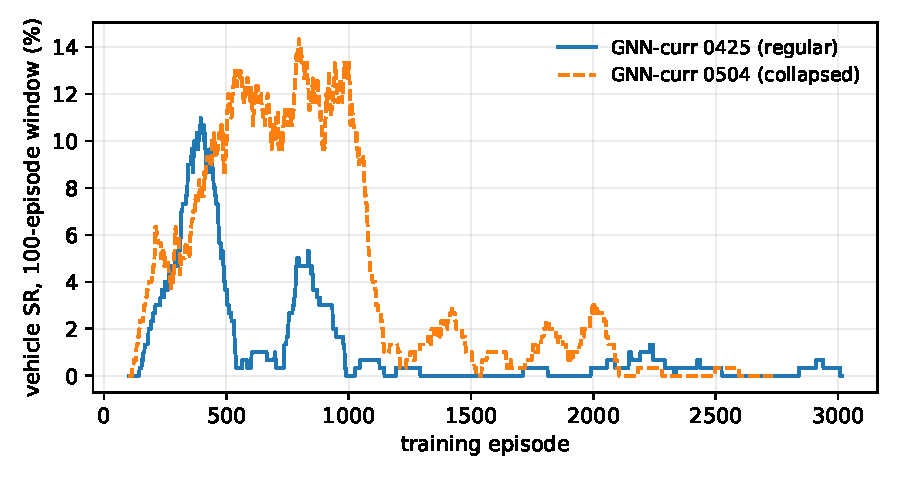
\includegraphics[width=0.85\textwidth]{pilot_collapse_timeseries}
  \caption{Windowed vehicle SR (100-episode window) for the two plain
  GNN-curriculum pilot runs. Run 0504 (dashed) sustains 10--14\% for
  $\approx$500 episodes, collapses near episode 1{,}100, and never
  recovers --- while ending with the \emph{highest} cumulative SR of the
  pilot (3.9\%, \cref{tab:pilot}). Cumulative aggregates inherit
  history; collapse detection requires windowed views.}
  \label{fig:pilot-collapse}
\end{figure}

% Sources for §5.2–5.4, §5.6: docs/thesis/data/campaign_consolidation.json,
% recomputed from disk 2026-07-15 by docs/thesis/scripts/
% consolidate_campaign.py (dedup, route_complete only, per class).
% GNN-B cells marked \todo until its training + the two GNN evals land.
\section{Campaign Integrity and Setup Recap}
\label{sec:integrity}

\Cref{tab:runmatrix} lists the campaign runs. All were launched on the
same trunk (commit \texttt{7defb03}) with seed 999; configuration diffs
confirm the cells differ only in the regime and critic-encoder flags
(\cref{sec:campaign}). The three completed training logs pass every
integrity condition of \cref{sec:metrics}: exactly six records per
episode throughout, zero malformed lines, zero non-finite values.

\begin{table}[t]
  \centering\small
  \caption{Campaign run matrix (all: 3M steps, Town03, seed 999, trunk
  \texttt{7defb03}). Realized level exposure is reported as
  easy/medium/hard shares of episodes.}
  \label{tab:runmatrix}
  \begin{tabular}{@{}llrrlll@{}}
    \toprule
    Cell & Run ID & Episodes & Records & Level mix (\%) & Integrity & Final eval \\
    \midrule
    MLP-curr.\ & 20260622\_171626 & 3220 & 19{,}320 & 32.5/45.8/21.6 & OK & 400 ep, done \\
    MLP-batch  & 20260623\_171855 & 3180 & 19{,}080 & 35.3/32.8/31.9 & OK & 400 ep, done \\
    GNN-curr.\ & 20260630\_181143 & 3293 & 19{,}758 & 32.4/37.4/30.1 & OK & \todo{pending} \\
    GNN-batch  & 20260714\_155209 & \multicolumn{4}{l}{\todo{training in progress}} & \todo{pending} \\
    \bottomrule
  \end{tabular}
\end{table}

The realized exposure matches the two designs: the batch run stays within
$\approx 2$ percentage points of the uniform $1/3$ per level, with all
three levels present within its first twenty episodes; the curriculum
runs concentrate easy/medium exposure early and reach hard only after
their unlocks (\cref{sec:sample-efficiency}), ending with hard shares of
21.6\% (MLP) and 30.1\% (GNN).

% ------------------------------------------------------------
\section{Sample Efficiency}
\label{sec:sample-efficiency}

\begin{figure}[t]
  \centering
  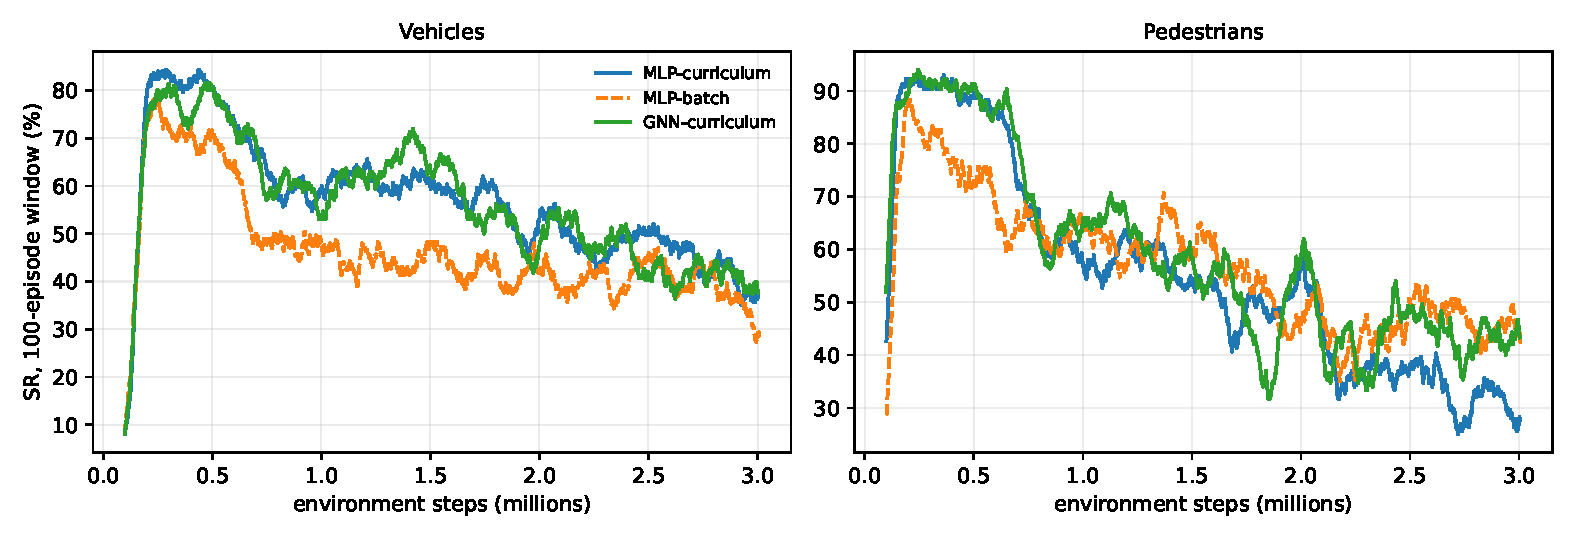
\includegraphics[width=\textwidth]{learning_curves}
  \caption{Windowed success rate (100-episode window) versus environment
  steps for the completed cells. \todo{Re-run
  \texttt{make\_fig5\_learning\_curves.py} to add GNN-batch when its
  training completes.} Important caveat: each curve is measured on that
  run's \emph{own concurrent level mix} --- gated for the curriculum
  cells, uniform for batch --- so vertical comparisons between arms are
  not like-for-like until the curriculum has unlocked all levels; the
  distribution-matched comparison is the final evaluation
  (\cref{sec:final-performance}).}
  \label{fig:learning-curves}
\end{figure}

\paragraph{Early phase: indistinguishable take-off.}
All three completed cells climb at the same speed: the 100-episode
windowed vehicle SR first crosses 30\% after 137--140K steps and 50\%
after 162--167K steps in every cell --- a spread of a few percent,
far inside noise. The notable part is \emph{what} each policy crossed it
on: the curriculum cells on easy-only exposure, the batch cell on the
full uniform mix including \SI{100}{m} routes. At equal budget, early
success-rate take-off was not the discriminating factor between regimes
in this campaign.

\paragraph{Unlock timing (curriculum cells).}
Medium unlocked at practically the same point in both curriculum runs
(episode 842 of 3220, 26.1\%, MLP; episode 860 of 3293, 26.1\%, GNN).
Hard, however, unlocked much earlier under the GNN critic: episode
1{,}910 (58.0\% of training) versus 2{,}286 (71.0\%) for MLP --- the
latter consistent with the 70\%-budget pressure cap firing rather than
the competence gate (\cref{sec:regimes}), while the GNN cell reached the
hard gate on competence. The result is visible in the exposure shares of
\cref{tab:runmatrix}: the GNN-curriculum policy saw $\approx 40$\% more
hard episodes than its MLP counterpart.

\paragraph{After the take-off.}
From $\approx 0.5$M steps the MLP-batch curve settles visibly below the
two curriculum curves (\cref{fig:learning-curves}), which track each
other closely; all curves drift downward late in training as the
curriculum mixes harden (curriculum cells) and as pedestrian windowed
success declines --- the within-run dynamics are analysed in
\cref{sec:behavior}.

% ------------------------------------------------------------
\section{Final Cumulative Performance}
\label{sec:final-performance}

\begin{table}[t]
  \centering\small
  \caption{Cumulative training metrics per cell (agent-level, \%;
  speed in km/h for vehicles, m/s for pedestrians).
  \todo{Add the GNN-batch row when its training completes.}}
  \label{tab:cumulative}
  \begin{tabular}{@{}lrrrrrrrr@{}}
    \toprule
    & \multicolumn{5}{c}{Vehicles} & \multicolumn{3}{c}{Pedestrians} \\
    \cmidrule(lr){2-6}\cmidrule(l){7-9}
    Cell & SR & s$+$t & coll. & off. & speed & SR & s$+$t & speed \\
    \midrule
    MLP-curr.\ & 57.28 & 30.48 & 8.84 & 3.41 & 10.2 & 56.59 & 42.56 & 1.96 \\
    MLP-batch  & 46.31 & 23.61 & 17.33 & 12.76 & 18.7 & 57.06 & 42.03 & 1.61 \\
    GNN-curr.\ & 56.55 & 20.84 & 13.37 & 9.23 & 18.0 & 60.50 & 38.58 & 1.91 \\
    GNN-batch  & \multicolumn{8}{l}{\todo{training in progress}} \\
    \bottomrule
  \end{tabular}
\end{table}

\begin{table}[t]
  \centering\small
  \caption{Final 400-episode evaluation, MLP pair (agent-level, \%).
  Scenarios: easy/medium/hard on Town03, test on Town05.
  \todo{Twin table for the GNN pair once its evaluations run.}}
  \label{tab:eval-mlp}
  \begin{tabular}{@{}llrrrrr@{}}
    \toprule
    Scenario & Cell & veh SR & veh s$+$t & veh coll. & veh off. & ped SR \\
    \midrule
    easy   & MLP-curr.\ & 60.33 & 28.00 & 7.33 & 4.33 & 58.00 \\
           & MLP-batch  & 41.33 & 28.33 & 18.00 & 12.33 & 58.67 \\
    medium & MLP-curr.\ & 51.67 & 36.00 & 9.00 & 3.33 & 40.67 \\
           & MLP-batch  & 31.00 & 27.67 & 25.33 & 16.00 & 41.67 \\
    hard   & MLP-curr.\ & 44.33 & 38.33 & 14.33 & 3.00 & 26.67 \\
           & MLP-batch  & 29.00 & 29.67 & 23.33 & 18.00 & 32.33 \\
    test   & MLP-curr.\ & 37.00 & 50.67 & 11.00 & 1.33 & 62.67 \\
           & MLP-batch  & 18.00 & 39.00 & 37.33 & 5.67 & 63.00 \\
    \midrule
    all    & MLP-curr.\ & 48.33 & 38.25 & 10.42 & 3.00 & 47.00 \\
           & MLP-batch  & 29.83 & 31.17 & 26.00 & 13.00 & 48.92 \\
    \bottomrule
  \end{tabular}
\end{table}

\paragraph{The primary contrast, MLP pair.}
On the distribution-matched final evaluation
(\cref{tab:eval-mlp}), the curriculum-trained vehicle policy completes
48.33\% of routes against 29.83\% for batch: $+18.5$ percentage points,
with the same sign in \emph{all four} scenarios ($+19.0$, $+20.7$,
$+15.3$, $+19.0$\,pp) and in cumulative training ($+11.0$\,pp,
\cref{tab:cumulative}). The margin is roughly two to four times the
same-seed replicate band of \cref{sec:iterations}, and its consistency
across scenarios, difficulty levels and measurement layers is what the
paired design can offer in place of seed replication
(\cref{sec:campaign}).

\paragraph{Two different ways to fail.}
The regimes produce recognizably different driving. The batch policy is
nearly twice as fast (18.7 vs.\ 10.2 km/h in training) but converts that
mobility into contact: collision 17.3\% vs.\ 8.8\% and offroad 12.8\%
vs.\ 3.4\% in training, widening to collision 26.0\% vs.\ 10.4\% at
evaluation. The curriculum policy fails mostly by stalling
(stuck$+$timeout 38.3\% vs.\ 31.2\% at evaluation). Neither profile
dominates the other on every axis --- the curriculum trades speed for
safety --- but on the strict success criterion the trade resolves
clearly in its favour.

\paragraph{Pedestrians: no regime effect.}
Pedestrian success is flat between arms everywhere: 56.6 vs.\ 57.1\% in
training, 47.0 vs.\ 48.9\% at evaluation, and within $\pm 6$\,pp in
every scenario. The training regime, in this platform, is a
vehicle-policy variable; the pedestrian task appears insensitive to task
ordering. Pedestrian failure structure is taken up in
\cref{sec:ped-limits}.

\paragraph{GNN-curriculum (training-only preview).}
Pending its evaluation, the GNN-curriculum cell lands within noise of
MLP-curriculum on headline SR (56.55 vs.\ 57.28\%) while redistributing
the failure mass: less stalling ($-9.6$\,pp stuck$+$timeout), more
contact ($+4.5$\,pp collision, $+5.8$\,pp offroad), and much higher
speed (18.0 vs.\ 10.2 km/h) --- closer to the batch cell's mobility with
curriculum-level success. If confirmed at evaluation, the critic encoder
would be shaping the \emph{risk profile} more than the success rate;
this thread is picked up in \cref{sec:arch-axis}.

\section{Behavioral Analysis}\label{sec:behavior}
% 2–2.5 pp: Q1->Q4 trajectories (data ready in campaign_consolidation.json:
% all cells decline Q1->Q4; MLP-B declines on a CONSTANT mix — real late
% degradation vs mix-hardening for C cells — disentangle), speed profiles,
% no_wp_steps, stuck causes; defensive-equilibrium case study (hazard gate)
% + P1xV1 coupling; ped windowed decline (fig) mix-confounded for C.

\section{Generalization: Town03 to Town05}
\label{sec:generalization}

The test scenario places the same policies on Town05 --- a squared-grid,
multi-lane layout structurally unlike Town03 (\cref{sec:carla-bg}) ---
for 100 episodes at \SI{80}{m} targets, with traffic as in training.
Three observations from the MLP pair (\cref{tab:eval-mlp}); the GNN pair
is \todo{pending evaluation}.

\paragraph{The ordering survives the map change.}
Curriculum completes 37.0\% of Town05 routes against batch's 18.0\%
($+19.0$\,pp) --- essentially the same margin as in-domain. The
absolute drop from the Town03 scenario average is nearly identical for
the two arms ($-15.1$\,pp from 52.1\% for curriculum; $-15.8$\,pp from
33.8\% for batch), so the curriculum advantage is not a Town03
idiosyncrasy: it transfers whole to roads never seen in training.
Read against hypothesis H2, the broader early coverage of the batch
regime bought it \emph{no} generalization edge --- if anything the
relative drop is worse from its lower base ($-47$\% vs.\ $-29$\%
relative).

\paragraph{Failure signatures amplify off-distribution.}
Each arm fails on Town05 the way it fails at home, only more so: the
curriculum policy stalls (stuck$+$timeout 50.7\%, its highest anywhere)
while keeping contact low (collision 11.0\%, offroad 1.3\%); the batch
policy crashes (collision 37.3\%, its highest anywhere). Novel roads
stress exactly the axis each policy already leaned on.

\paragraph{Pedestrians transfer easily.}
Pedestrian success on Town05 (62.7 vs.\ 63.0\%) exceeds both arms'
Town03 hard-level results by $\approx 30$\,pp --- the \SI{80}{m} test
routes are more feasible than Town03's \SI{100}{m} hard routes, pointing
again at route feasibility rather than policy generalization as the
pedestrian bottleneck (\cref{sec:ped-limits}).

\section{Architecture Axis: MLP vs GNN Critic}\label{sec:arch-axis}
% 1.5–2 pp (H3): does the C-vs-B contrast replicate on both architectures?
% arch x regime interaction; link to April pilot signature.

\section{Pedestrian Structural Limits}\label{sec:ped-limits}
% 1–1.5 pp: route feasibility (under_target/too_short/sidewalk_fallback),
% medium/hard collapse: environment vs policy limits.

\section{Findings versus Hypotheses}\label{sec:findings}
% 0.5–1 pp: H1/H2/H3 -> supported/rejected/partial per axis.

% ============================================================
% Chapter 6 — Discussion (target 4–5 pp)
% ============================================================
\chapter{Discussion}
\label{ch:discussion}

\todo{Chapter not started. Skeleton below per the outline.}

\section{What Task Ordering Changes (and What It Does Not)}\label{sec:ordering}
% Interpretation of the 4 comparison axes.

\section{Parallel Task Coverage Revisited}\label{sec:ptc-revisited}
% What the evidence says about interactions, correlated samples,
% non-stationarity.

% --- §6.3–6.4 drafted 2026-07-14 (results-independent; re-read after
%     Ch. 5 is final to update the n-per-cell statement). ---
\section{Threats to Validity}
\label{sec:threats}

\paragraph{Simulator non-determinism under identical conditions.}
The dominant threat, quantified rather than assumed: three full-length
runs of byte-identical code, configuration and seed produced cumulative
vehicle success rates ranging 52.2--62.4\% (\cref{sec:iterations}).
CARLA under multi-agent load is not run-to-run deterministic even in
synchronous mode with all seeds fixed. Every effect in this thesis is
therefore read against this $\sim$10\,pp band: differences within it are
never attributed to an experimental factor, whatever their direction. The
band was measured on the pre-campaign trunk at training level; it is
assumed representative for campaign-era runs, which is itself an
approximation.

\paragraph{Sample size.}
Each cell contains a single run: the design was reduced from three paired
seeds per cell to one for compute reasons, a decision declared in
\cref{sec:campaign}. Every conclusion therefore rests on paired
contrasts, not on estimated distributions. Seed pairing and
byte-identical configurations make the contrasts internally clean, and
the primary contrast carries one built-in replication --- it is observed
independently under both critic architectures --- but no formal
statistical inference is possible at this $n$, and none is claimed. The
mitigations are the replicate band above and consistency checks ---
direction agreement across difficulty levels, evaluation scenarios,
agent classes, and measurement layers --- rather than significance
tests.

\paragraph{Evaluation noise.}
The final evaluation uses 100 episodes per scenario, i.e.\ 300 vehicle
records; at mid-range success rates the binomial standard error alone is
$\approx$3\,pp per scenario, before accounting for the within-episode
correlation of the three vehicles, which lowers the effective sample
further. Scenario-level differences of a few points are therefore not
individually meaningful; only patterns across scenarios are interpreted.

\paragraph{Reward--curriculum coupling.}
The reward function was tuned through gate iterations run mostly on
easy-locked configurations (\cref{sec:gate}), so the trunk's shaping may
be implicitly biased toward short routes. Both regimes share the
identical reward, so the primary contrast remains internally valid; the
caveat applies to interpreting \emph{absolute} performance on hard
routes, and to the possibility that a differently tuned reward would
shift the two regimes differently.

\paragraph{Single map pair.}
Generalization is measured on exactly one transfer, Town03 $\to$ Town05.
The two layouts differ in kind (\cref{sec:carla-bg}), which makes the
test meaningful, but claims are limited to this pair; no evidence is
offered that the ranking of regimes transfers to other maps, traffic
compositions, or weather conditions.

\paragraph{Measurement history.}
The evaluation pipeline itself failed validity once
(\cref{sec:bugs}), and the route-length defect silently redefined the
task distribution for a whole era of experiments. Both were caught by
integrity signals (implausibly regular outputs; missing per-agent logs).
The protocol now in place --- integrity checks, paired configurations,
recomputation from raw logs --- was built in response, but the general
lesson stands as a threat class: in a custom platform, apparent effects
must first survive the question ``is the instrument measuring what it
claims?''

\paragraph{Pedestrian route feasibility.}
Pedestrian results at medium/hard difficulty are confounded by a
structural environment limit: Town03's sidewalk topology often cannot
support the nominal route targets (\cref{sec:routes}). \Cref{sec:ped-limits}
separates environment-attributable from policy-attributable failure, and
pedestrian-side regime conclusions are restricted accordingly.

% ------------------------------------------------------------
\section{Scope Limitations}
\label{sec:scope}

Beyond threats to internal validity, the design deliberately fixes
several dimensions; findings should not be read beyond them.

\begin{itemize}
  \item \textbf{Actor architecture is fixed.} Both classes use MLP
        actors throughout; only the \emph{critic encoder} varies (MLP
        vs.\ GNN, training-side only). This thesis makes no claim about
        policy-network architecture, and the GNN axis speaks only to
        value estimation under CTDE.
  \item \textbf{The shared-world frame is not ablated.} Parallel task
        coverage (\cref{sec:parallel-coverage}) is the fixed frame of
        both arms, not a treatment: there is no 1-agent-per-world
        control, so its causal contribution to sample efficiency is
        characterized, not isolated.
  \item \textbf{Privileged observations, no perception.} Agents observe
        curated state features (\cref{sec:obs-actions}), not sensors.
        All findings concern decision-making under interaction;
        nothing follows for camera- or lidar-based pipelines.
  \item \textbf{One algorithm, one platform version.} MAPPO on
        RLlib~2.10.0 and CARLA~0.9.16 throughout. Regime effects are
        conditional on this stack; other algorithms may interact with
        task ordering differently.
  \item \textbf{Difficulty is route length only.} The configuration
        defines traffic-density and mixed difficulty families, but they
        are unused (\cref{sec:campaign}); ``difficulty'' in every claim
        means target route length at fixed traffic.
  \item \textbf{Fixed population.} Always 3 vehicles $+$ 3 pedestrians;
        no scaling evidence in either direction.
  \item \textbf{Pedestrian route generation.} The sidewalk-chain planner
        with its crossing cap is part of the platform being studied; its
        known feasibility limits bound what pedestrian policies can
        express, independently of training regime.
\end{itemize}

% ============================================================
% Chapter 7 — Conclusions & Future Work (target 2–3 pp)
% ============================================================
\chapter{Conclusions and Future Work}
\label{ch:conclusions}

\todo{Chapter not started.}

\section{Conclusions}\label{sec:conclusions}
% Answer to the research question + contributions.

\section{Future Work}\label{sec:future}
% Architectural extensions (GAT = GNN+attention, PopArt — flags already in
% the infrastructure), scaling to 100+ agents (application vision),
% adaptive/automatic curricula, pedestrian route-generation fix.


% ----------------- Appendices -------------------------------
\appendix
% ============================================================
% Appendices A–D
% Status 2026-07-14: A, B, D full draft; C awaits the campaign.
% Sources: project registry (CLAUDE.md / docs/EXPERIMENT_REGISTRY.md),
% config snapshots in latex/configs/ (copied from carla_core/configs
% on 2026-07-14), hardware read from the machine.
% ============================================================

\chapter{Experiment Registry (Condensed)}
\label{app:registry}

\Cref{tab:registry} lists every evaluated candidate with its run
identifier, verdict, and headline outcome. Development-phase A/B runs are
$3\times10^{5}$ steps, seed 999, easy-locked unless noted; deltas are
versus the paired baseline of their era (\cref{sec:gate}) and are not
comparable across environment versions (\cref{sec:bugs}). The full
registry, with per-candidate mechanisms and pseudocode, is maintained in
the repository (\texttt{docs/EXPERIMENT\_REGISTRY.md}).

\begin{small}
\begin{longtable}{@{}p{3.1cm}p{2.8cm}p{2.0cm}p{5.6cm}@{}}
  \caption{Condensed experiment registry. SR = vehicle success rate,
  s$+$t = stuck$+$timeout, EV = critic explained variance.}
  \label{tab:registry}\\
  \toprule
  Candidate & Run ID & Verdict & Outcome \\
  \midrule
  \endfirsthead
  \toprule
  Candidate & Run ID & Verdict & Outcome \\
  \midrule
  \endhead
  C0 diagnostics & --- & adopted & episode-log instrumentation; measurement only \\
  C1 route-aware obs & --- & adopted & geometric route features (44D era) \\
  C2v2-A movement reward & 20260514\_001215 & not promoted & SR up but s$+$t worsened \\
  D1 obs/reward & 20260514\_073353 & rejected & SR down, s$+$t up \\
  D2 reward shaping & 20260514\_095921 & promoted & anti-stall block of \cref{sec:rewards} \\
  D1$+$D2 & 20260514\_133823 & rejected & worse than D2 alone \\
  D2-Safety & 20260514\_155151 & rejected & SR down, no safety gain \\
  D3 early stuck termination & 20260514\_190424 & rejected & SR $-2.9$\,pp, s$+$t $+7.1$\,pp \\
  Easy-only path lock & 20260514\_211642 & evidence only & exploratory, no gate \\
  H1$+$H1.1 value-loss repair & 20260515\_175921 & retained (gate fail) & EV $0 \to 0.87$; collision $+3.3$\,pp \\
  H2 discount $0.99 \to 0.997$ & 20260515\_211055 & retained (falsified) & collision $+5.2$\,pp, timeout$\to$collision $\approx$1:1 \\
  H3 entropy schedule (step-based) & 20260516\_144007 & gate fail & mechanism confirmed (entropy $4.78 \to 3.25$); deltas within noise \\
  R3 collision penalty $\times 10$ & 20260516\_200545 & retained (falsified) & collision flat ($-0.2$\,pp): perception limit, not reward weight \\
  R1 progress-guard removal & 20260517\_134652 & promoted & SR $+4.7$\,pp, s$+$t $-3.5$\,pp, coll.\ $-1.5$\,pp \\
  R2 gated steering bonus & 20260517\_164707 & not promoted & SR $-1.9$\,pp, offroad $+3.2$\,pp \\
  Route-length bugfix & 20260517\_212109 & adopted (bug fix) & $\approx +50$\,pp SR: task-distribution change (\cref{sec:bugs}) \\
  Route-seed fix & --- & adopted (bug fix) & restores A/B route pairing (\cref{sec:bugs}) \\
  O1$+$O2 observability (47D) & 20260518\_195947 & adopted & healthy baseline: easy-locked SR $\approx 79$\%, EV 0.983 \\
  Entropy schedule (fraction-based) & 20260520\_133747 & promoted & stable mechanism; baseline for later gates \\
  Ped route$+$pace bundle & 20260525\_091300 & partial & ped SR flat but pace out of band; vehicle ripple (stuck $+4.7$\,pp) \\
  V3 pace-band retune & 20260525\_125127 & rejected & overshoot worse (2.64\,m/s); Q4 SR decline \\
  V1 hazard-gate $0.75 \to 0.85$ & 20260525\_162428 & promoted & 5/5: SR $+2.3$\,pp, s$+$t $-3.0$\,pp, coll./off.\ improved \\
  Unlock-path training at 3M & 20260525\_205912 & completed & first full-horizon curriculum run (V1$+$P1--P3 stack) \\
  Evaluation-pipeline fixes & commit \texttt{d0731ca} & adopted (tooling) & four coupled eval bugs (\cref{sec:bugs}); no training change \\
  \texttt{route\_short} as success & 20260529\_122522 & reverted & violated the success criterion; vehicle regression suspected, unresolved ($n=1$) \\
  Post-revert confirmation & 20260610\_192146 & pass & regression not reproduced; third member of the replicate band \\
  Crosswalk cap $8 \to 3$ & 20260622\_132848 & promoted & SR $+9.2$\,pp, coll.\ $-2.3$\,pp, off.\ $-2.2$\,pp, ped flat (hard-locked A/B) \\
  \bottomrule
\end{longtable}
\end{small}

\chapter{Full Configuration}
\label{app:hyperparams}

The three configuration files below are verbatim snapshots (2026-07-14)
of the campaign trunk; the per-run \texttt{run\_config.json} written at
launch is the authoritative record for any individual run and was used to
verify that campaign cells differ only in the two experimental flags
(\cref{sec:campaign}). The traffic and mixed level families in
\texttt{levels.yaml} are defined but unused in this thesis.

\section*{\texttt{train\_mappo.yaml}}
{\scriptsize\verbatiminput{configs/train_mappo.yaml}}

\section*{\texttt{curriculum\_batch.yaml}}
{\scriptsize\verbatiminput{configs/curriculum_batch.yaml}}

\section*{\texttt{levels.yaml}}
{\scriptsize\verbatiminput{configs/levels.yaml}}

\chapter{Per-Run Results}
\label{app:per-seed}
\todo{Complete per-run tables for the four campaign runs (populate once
the $2\times2$ matrix is closed: full metric catalogue per cell, per
class, per level, training $+$ final evaluation).}

\chapter{Reproducibility}
\label{app:repro}

\paragraph{Software stack.}
CARLA 0.9.16 (server and Python API); Python 3.11.9; PyTorch 2.7
(CUDA 12.6); Ray/RLlib 2.10.0. Training and simulator run on the same
machine.

\paragraph{Hardware.}
All runs were executed on a single laptop-class machine: Intel Core
i7-10870H (8 cores / 16 threads), \SI{16}{GB} RAM, NVIDIA GeForce RTX
3080 Laptop GPU (\SI{8}{GB}), Windows 11. The resource envelope is part
of the study's design constraints: it motivates the $3\times10^{5}$-step
diagnostic budget of the gate protocol (\cref{sec:gate}) and the
$n=3$-seed ceiling of the campaign.

\paragraph{Code version.}
The campaign trunk is commit \texttt{7defb03} (merge of the crosswalk-cap
branch, 2026-06-22); later commits up to the writing of this thesis touch
documentation and visualization tooling only. Each run directory stores
its own \texttt{run\_config.json} (exact configuration), checkpoints, and
\texttt{episodes.jsonl} (raw agent-level records) from which every number
in this thesis is recomputed.

\paragraph{Commands.}
Training (one per campaign cell; the four cells vary only
\texttt{--mode} and \texttt{--use-gnn}):
\begin{quote}\small\ttfamily
python -m carla\_core.training.train\_carla\_mappo --mode curriculum
--difficulty path --timesteps 3000000 --seed 999 [--use-gnn]
\end{quote}
Training writes a \texttt{final\_eval\_job.json} into the run directory;
the final 400-episode evaluation (\cref{sec:eval-pipeline}) is launched
with:
\begin{quote}\small\ttfamily
python -m carla\_core.training.evaluate\_carla\_mappo --job
<run\_dir>/final\_eval\_job.json
\end{quote}
Static recomputation from logs and thesis figures:
\begin{quote}\small\ttfamily
python carla\_core/scripts/verify-check-test/evaluate\_run\_static.py \\
python docs/thesis/scripts/make\_pilot\_collapse\_fig.py \\
python docs/thesis/scripts/make\_fig3\_route\_examples.py
\end{quote}

\paragraph{Seeds.}
Campaign: a single experiment seed (999), paired across all four cells.
April pilot era: seed 42. Per-agent route seeds derive
deterministically from the experiment seed (\cref{sec:seeding}). Note
that seeding does not make CARLA runs identical (\cref{sec:threats});
reproducibility here means reproducing the \emph{distribution} of
outcomes and every reported aggregate from the archived logs.


% ----------------- Bibliography -----------------------------
\printbibliography[heading=bibintoc]

\end{document}
